% % % % % % % % % % % % % % % % % % % % % % % % % % % % % % % % % % % % % % % % % % % %
%                                                                                     %
% Short Sectioned Assignment LaTeX Template Version 1.0 (5/5/12)                      %
% This template has been downloaded from: http://www.LaTeXTemplates.com               %
%                                                                                     %
% Original author:  Frits Wenneker (http://www.howtotex.com)                          %
%                                                                                     %
% Modified by: Fco Javier Sueza Rodríguez (fcosueza@disroot.org)                      %
%                                                                                     %
% Changes:                                                                            %
%           - Document type scrarticle                                                %
%           - Use babel-lang-spanish package and marvosym                             %
%           - Use hyperref, enumitem and tcolorbox                                    %
%           - Use fancyhdr package an configure it                                    %
%           - Use Time New Roman (mathptmx), Helvetic and Courier fonts               %
%                                                                                     %
% License: CC BY-NC-SA 3.0 (http://creativecommons.org/licenses/by-nc-sa/3.0/)        %
%                                                                                     %
% % % % % % % % % % % % % % % % % % % % % % % % % % % % % % % % % % % % % % % % % % % %

%-----------------------------------------------%
%	              Packages                  %
%-----------------------------------------------%

\documentclass[bibliography=totoc]{scrarticle}

% ---- Text Input/Output ----- %

\usepackage[T1]{fontenc}
\usepackage[utf8]{inputenc}
\usepackage{mathptmx}
\usepackage[scaled=.92]{helvet}
\usepackage{courier}
\usepackage[indent=12pt]{parskip}

\usepackage{geometry}
\geometry{verbose,tmargin=3cm,bmargin=3cm,lmargin=2.5cm,rmargin=2.5cm}

% ---- Language ----- %

\usepackage[spanish]{babel}
\usepackage{marvosym}

% ---- Another packages ---- %

\usepackage{amsmath,amsfonts,amsthm}
\usepackage{graphics,graphicx}
\usepackage{tcolorbox}
\usepackage{hyperref}
\usepackage{enumitem}
\usepackage{fancyhdr}
\usepackage{float}

%--------------------------------------------------------------------%
%                      Customizing Document                          %
%--------------------------------------------------------------------%

% -------------- Customize headers and footers---------------------- %

\pagestyle{fancy}

\fancyhead[]{}
\fancyfoot[L]{}
\fancyfoot[C]{}
\fancyfoot[R]{\thepage}

\renewcommand{\headrulewidth}{0pt} % Remove header underlines
\renewcommand{\footrulewidth}{0pt} % Remove footer underlines

% Needed to get first page footer correctly
\fancypagestyle{plain}{
    \fancyhf{}
    \fancyfoot[R]{\thepage}
}

% --------------------- Packages Configuration --------------------- %


\hypersetup{
    colorlinks=true,
    linkcolor=black,
    urlcolor=magenta
}

\setcounter{secnumdepth}{4}
\setcounter{tocdepth}{4}
\graphicspath{{./images/}}

\setlength{\headheight}{13.6pt} % Customize the height of the header
\numberwithin{figure}{section} % Number figures within sections

% ------------------------ New Commands ----------------------------- %

\newcommand{\horrule}[1]{\rule{\linewidth}{#1}} % Create horizontal rule command


%----------------------------------------------------------------------------------------
%	TÍTULO Y DATOS DEL ALUMNO
%----------------------------------------------------------------------------------------

\title{
\vspace{10ex}
\normalfont \normalsize
\huge \textbf{Proyecto Web: SolucionesVecinales}
}
\author{Francisco Javier Sueza Rodríguez}
\date{\normalsize\today}

\glsenablehyper
\makeglossaries
\loadglsentries{glos}

%----------------------------------------------------------------------------------------
%                                     DOCUMENTO
%----------------------------------------------------------------------------------------
\begin{document}


\maketitle

\thispagestyle{empty}

\vspace{75ex}

\begin{center}
    \begin{tabular}{l l}
        \textbf{Centro}: & IES Aguadulce \\
        \textbf{Ciclo Formativo}: & Desarrollo Aplicaciones Web (Distancia)\\
        \textbf{Asignatura}: & Proyecto DAW\\
    \end{tabular}
\end{center}

\newpage

\begingroup
\hypersetup{linkcolor=black}
\tableofcontents
\endgroup

\newpage

\begingroup
\hypersetup{linkcolor=black}
\listoffigures
\listoftables
\endgroup

\newpage

\section{Introducción}

\subsection{Presentación}
En este documento se detalla el proyecto final desarrollado para el \textbf{CFGS Desarrollo de Aplicaciones Web} en el \textbf{IES Aguadulce}. El proyecto elegido ha sido una aplicación web para la \textbf{gestión y administración de comunidades de vecinos}, llamada \textbf{SolucionesVecinales}.

El objetivo de esta aplicación es facilitar la \textbf{gestión de comunidades de vecinos} por parte tanto de los administradores de la propiedad como de los inquilinos o propietarios, ofreciéndose de \textbf{forma gratuita} y poniendo especial énfasis en las \textbf{accesibilidad} y \textbf{facilidad de uso}, con una interfaz web amigable y accesible desde cualquier dispositivo que disponga una navegador web.

La aplicación trabaja con \textbf{3 tipos diferentes de usuarios}, incluyendo administradores, inquilinos y visitantes, siendo el público objetivo los administradores de propiedad y presidentes de comunidad así como todos los inquilinos y propietarios de las comunidades de vecinos. Los diferentes usuarios tendrán diferentes permisos y responsabilidades.

A lo largo de este documento, desgranaremos todas los requisitos de la aplicación, el diseño elegido y todos los detalles del proceso de desarrollo y testeo.

\subsection{Contexto}
Esta aplicación es un \textbf{proyecto personal} que se ha decidido realizar tras el análisis de diferentes aplicaciones similares y ver determinadas carencias que pueden dificultar la inclusión de todos los potenciales usuarios. Hay que tener en cuenta, que los usuarios objetivos son un grupo muy heterogéneo donde podemos encontrar personas con diferente formación, conocimientos sobre tecnologías o con problemas de accesibilidad, así como gente con dificultades económicas.

Por este motivo, se ha decidido realizar una \textbf{aplicación gratuita}, centrándonos en la \textbf{accesibilidad} y \textbf{facilidad de uso}, que ayude a cualquier potencial usuario a usar la aplicación e implicarse en la gestión de su comunidad de vecinos. 

\subsection{Planteamiento del Problema}
La gestión de comunidades de vecinos es una tarea compleja que requiere realizar un conjunto de gestiones administrativas asegurando la participación de los vecinos y de una forma transparente. En este aspecto, nuestra aplicación debería permitir que se realicen las siguientes tareas:

\begin{itemize}
	\item \textbf{Gestión de documentos}: gestión de los documentos generados en los diferentes procesos, como resolución de incidencias, documentos sobre juntas vecinales, etc. Permitiendo que estos puedan ser accedidos por todos los vecinos de la comunidad.
	
	\item \textbf{Reserva de espacios comunes}: automatizar la reserva y gestión de espacios comunes permitiendo a los vecinos reservar o cancelar reservas de dichos espacios, así como acceder a una lista con los espacios y el estado actual de reserva.
	
	\item \textbf{Gestión de Incidencias}: se debe permitir la creación de incidencias por parte de los vecinos así como su administración por parte del presidente de la comunidad o el administrador de fincas.
	
	\item \textbf{Gestión de Usuarios y Comunidades}: la aplicación debe permitir la creación, baja, actualización y consulta de usuarios con diferentes roles así como de comunidades de vecinos.
	
	\item \textbf{Gestión de Finanzas}: la aplicación debe realizar, de forma automática, cálculos para administrar económicamente la comunidad, calculando el balance anual a partir de las cuotas que se están pagando y las diferentes facturas que se han pagado.
\end{itemize}

Además de estas tareas, hay que garantizar la seguridad de la información almacenada, ya que es información sensible, así como que el proceso para realizar estas tareas sea sencillo e intuitivo, además de accesible. 

\subsection{Visión General}
Este documento se compone de 6 secciones principales que tratan diferentes aspecto del proyecto. Para facilitar al interesado la navegación por éste, vamos a explicar brevemente en que consiste cada sección del documento:

\begin{itemize}
	\item \textbf{Análisis de Requisitos}: en esta sección se especifican los requisitos, tanto funcionales como no funcionales de la aplicación, especificando que es lo que se quiere conseguir con este proyecto y cuales son las restricciones que vienen impuestas. bien por el problema a tratar o por los propios requisitos.
	
	\item \textbf{Hardware y Software Necesario.}: en esta sección se especifica el hardware necesarios para realizar el desarrollo y poner en funcionamiento la aplicación así como el software que se va a necesitar para este mismo propósito. También se especifica el presupuesto y los costes de hosting para la aplicación.
	
	\item \textbf{Casos de Uso}: en esta sección se realiza un análisis de los principales casos de uso, empleando diferentes diagramas, así como una descripción más detalladas de los casos de uso generales.
	
	\item \textbf{Diseño de la Interfaz}: en esta sección se especifica el diseño de la interfaz de usuario, mostrando todas las páginas de la aplicación así como la relación entre estas y sus diferentes elementos.
	
	\item \textbf{Diseño de la Base de Datos}: en este apartado se especifica el diseño de la base de datos, empleando un esquema Entidad-Relación así como el paso a tablas de ésta, explicando los puntos que sean oportunos sobre las decisiones de diseño tomadas. Además, se incluyen dos script, uno para la creación de la base de datos y otro para poblarla con datos.
	
	\item \textbf{Diagrama de Componentes}: en esta sección se muestra el diagrama de componentes de la aplicación, poniendo de relieve la arquitectura de la aplicación así como las interacción entre los diferentes elementos y sistemas.
\end{itemize}



\section{Análisis de Requisitos}

\subsection{Introducción}
En esta sección se va definir la \textbf{especificación de requerimientos} que establece los requisitos funcionales y no funcionales de la aplicación SolucionesVecinales, realizando una análisis del funcionamiento esperado de aplicación y estableciendo unos límites para el diseño de ésta.

\subsubsection{Propósito}
El propósito de esta sección es \textbf{establecer los requisitos}, tanto funcionales como no funcionales, de la aplicación que se va a desarrollar, realizando una \textbf{análisis exhaustivo de su funcionamiento} y estableciendo las restricciones necesarias para que la aplicación cumpla su funcionalidad de forma correcta, segura y eficiente. Estos requisitos nos ayudarán a planificar el proceso de desarrollo así como a tomar las decisiones oportunas durante el diseño de la aplicación.

Esta sección va dirigida principalmente al \textbf{equipo de desarrollo}, que serán los encargados de diseñar la aplicación a partir de los requerimientos y restricciones establecidos en este documento, aunque teniendo en cuenta que también esta incluido en el documento del proyecto en general cabe la posibilidad de que tengan acceso a él otros interesados, como por ejemplo, posibles inversores.

\subsubsection{Alcance}
Nuestro producto se llama \textbf{SolucionesVecinales} y es una aplicación web para la \textbf{gestión de comunidades de vecinos}. El fin de nuestra aplicación es ayudar a todos los integrantes en una comunidad de vecinos a realizar diferentes gestiones relacionadas con las administración de su comunidad, de forma simple y sencilla. 

Es una aplicación que se \textbf{ofrece de forma gratuita}, cuya meta principal es llegar al mayor número de usuarios, implementando buenas \textbf{políticas de accesibilidad} y ofreciendo una \textbf{interfaz sencilla} e \textbf{intuitiva} que pueda usar cualquiera persona, incluso aquellos que no están familiarizados con las nuevas tecnologías. 

Partiendo de esta base, la aplicación deberá \textbf{ayudar a realizar las tareas} más comunes en las que deben participar los vecinos en una comunidad, como el acceso de documentos, creación de incidencias, consulta de las cuentas de la comunidad,  reserva de espacios comunes, etc.

\subsubsection{Definiciones, Siglas y Abreviaturas}
Las definiciones, siglas y abreviaturas se incluyen al final del documento, dentro de un Glosario, donde se incluyen todos los términos tanto de esta sección como del resto de secciones.

\subsubsection{Referencias}
La referencias, al igual que el glosario, tanto de esta sección como del resto de secciones se incluyen al final de documento, para no duplicar secciones. Además, en cada texto que haga referencia a alguna página o documento, se incluirá la cita adecuada apunta a dicha referencia, para facilitar su acceso.


\subsubsection{Visión General}
Esta sección se divide a su vez en 4 secciones, incluyendo la actual. Cada sección describe un aspecto diferentes de los requisitos del software y son las siguientes:

\begin{itemize}
	\item \textbf{Introducción} (Sección 2.1): en esta primera sección se realiza una introducción tanto al software como a este documento, explicando su propósito, alcance, etc...
	
	\item \textbf{Descripción General} (Sección 2.2): en esta sección se realiza una descripción del software que se va a desarrollar, incluyendo su funcionalidad, restricciones, características de los usuarios potenciales, interfaces, etc. Nos sirve como base para especificar los requisitos en el siguiente apartado.
	
	\item \textbf{Requerimientos Específicos} (Sección 2.3): en la tercera sección vamos a establecer los requisitos específicos del software, extraídos de la descripción general y separados en requisitos funcionales y no funcionales.
	
	\item \textbf{Requerimientos de Documentación} (Sección 2.4): en esta sección de la parte de requisitos se especifican los requisitos de documentación que va a tener el software, incluyendo manuales, ayuda en línea, instalación, etc.
\end{itemize}

\subsection{Descripción General}
En esta sección se van a describir todos los factores y restricciones que afectan al producto, estableciendo una base para la definición de los requisitos específicos en la siguiente sección, incluyendo una perspectiva general del producto, así como las restricciones que se deben aplicar en su diseño.

\subsubsection{Perspectiva del Producto}
En primer lugar vamos a realizar una descripción del producto, especialmente de las diferentes interfaces que se van a emplear y su interacción con los diferentes elementos y sistemas con los que deberá interactuar nuestro software.

\paragraph{Interfaz de Usuario}
~\\\\
\-\ \-\ \-\ Debido a que las especificaciones sobre al interfaz de usuario son más extensas, se han incluido como un anexo. Estas especificaciones se pueden consultar, en concreto, en el \hyperref[sec:apenA]{Anexo A}.


\paragraph{Interfaces con Hardware}
~\\\\
\-\ \-\ \-\ Nuestro software \textbf{no interactúa directamente con el hardware} de los dispositivos, ya que en la parte del cliente la interacción se realiza con el navegador web, mientras que en la parte del servidor la interacción se realiza con el servidor web. Estos, a su vez, realizarán las interacciones necesarias con el SO.

Sí cabe destacar en esta sección, ya que no veo otra donde pueda incluir esta información, que \textbf{nuestro software} se deberá usar desde \textbf{cualquier dispositivo} que cuente con un \textbf{navegador web}, por lo que deberá realizarse el diseño teniendo esto en cuenta. Realmente esto solo afecta a la estética de la aplicación en cada dispositivo, y no en su funcionamiento, y tampoco requiere del empleo de ninguna interfaz específica, por lo que solo afectará a la \textbf{interfaz de usuario}. 


\paragraph{Interfaces con Software}
~\\\\
\-\ \-\ \-\ Nuestra aplicación \textbf{no usa ninguna interfaz externa} para comunicarse con ningún software externo. 

La \textbf{única interacción} que cabe mencionar es la que realiza la parte de cliente de nuestra aplicación con el \textbf{navegador web} del usuario, aunque en este aspecto no se emplea ninguna interfaz específica para llevar a cabo esta interacción, si no que se realiza a través de los lenguajes empleados para desarrollar el propio cliente, como HTML, CSS, Javascript, etc.

En el \textbf{lado del servidor}, nuestra aplicación se ejecutará en un servidor web, aunque como hemos comentado, no se va a emplear ninguna interfaz para comunicarse con el. Para ejecutar nuestra aplicación vale cualquier servidor web, aunque si hay que tener en cuenta un detalle, y es que cuando la aplicación se este \textbf{ejecutando en producción}, el servidor deberá tener soporte para \gls{SSL}, ya que nuestra aplicación va a emplear el protocolo \textbf{HTTPS} para comunicarse.

\paragraph{Interfaces de Comunicación}
~\\\\
\-\ \-\ \-\ Para que nuestra aplicación funciones correctamente \textbf{necesita comunicarse mediante una red}, ya sea local o internet, realizando al comunicación entre nuestro cliente, con el navegador del usuario, y nuestro servidor. Para llevar a cabo esta comunicación, se va a emplear el protocolo \gls{HTTP}.

El \textbf{protocolo HTTP} es el estándar para la comunicación web desde hace muchos años, inventado por Tim Berners-Lee en 1989, es un protocolo de la capa de aplicación que es la base de la comunicación en la World Wide Web. \cite{wiki01}

En este documento \textbf{no vamos a discutir} ni exponer las \textbf{especificaciones} de todo el \textbf{protocolo HTTP}, ya que el uso de este protocolo se va a realizar mediante funciones predefinidas por los lenguajes sin tener que preocuparnos de como se implementa dicho protocolo, aunque si vamos a comentar un par de puntos que si conviene tener en cuenta.

En primer lugar, hay que hablar de los \textbf{métodos HTTP}, que son un conjunto de ``verbos'' que se usan para solicitar, desde el cliente, diferentes tipos de acciones que debe realizar el servidor, como puede ser mandar información, modificarla, eliminarla, etc... Los verbos HTTP que podemos emplear son GET, HEAD, POST, PUT, DELETE, CONNECT, OPTIONS, TRACE y PATCH. \cite{mdn01}

Cada método tiene una funcionalidad diferente, con diferentes ventajas e inconvenientes, pero nosotros no vamos a describir aquí todos, si no que nos vamos a centrar en los únicos que nos interesan y que vamos a usar en nuestra aplicación, que son \textbf{GET}, \textbf{POST}, \textbf{PUT} y \textbf{DELETE}. Las principales características de estos métodos son las siguientes:

\begin{itemize}
	\item \textbf{GET}: este método se emplea para realizar \textbf{peticiones al servidor} sobre el \textbf{estado representacional de algún recurso}. Las peticiones con este método se pueden almacenar en una caché y la información de la petición se pueden ver en la URL que se le pasa al servidor. Además es un método seguro, ya que no altera información del servidor e \gls{idempotente}. \cite{mdn02}
	
	\item \textbf{POST}: este método se emplea para \textbf{enviar información al servidor}, la cual se envía en el \textbf{cuerpo de la petición}. El resultado puede ser alguna acción realizada por el servidor como comprobar que los datos son correctos, crear nuevos datos o modificarlos. Es un método no seguro, ya que modifica información en el servidor, y tampoco es cacheable ni idempotente. \cite{mdn03} 
	
	\item \textbf{DELETE}: con éste método se le indica al servidor que elimine un recurso específico. Este método no es seguro ni cacheable, pero si es idempotente. \cite{mdn04}
	
	\item \textbf{PUT}: este método crea o modifica un recurso en el servidor añadiendo el contenido en el cuerpo de la solicitud. La principal diferencia entre PUT y POST es que PUT es idempotente. \cite{mdn05}
\end{itemize}

Estos métodos tienen que tenerse claros en el proceso de desarrollo, ya que la \gls{API} de nuestra aplicación deberá manejar correctamente las diferentes peticiones que se hagan con estos métodos, y nuestro cliente deberá realizar las peticiones con el método adecuado. 

Cabe destacar que nuestra aplicación usara \textbf{HTTPS}, aunque esto no va a afectar en como van a tratarse los métodos ni a procesarse, sino en como se realizará la conexión, que tiene más que ver con la configuración del servidor.

Por otro lado, debemos hablar de los \textbf{códigos HTTP de respuesta}. Estos códigos son los que deberá responder el servidor a las diferentes peticiones que realice el cliente. No vamos a explicar cuales son todos los códigos, ya que sería muy extenso, simplemente comentar que en todo momento se deberá enviar el código adecuado al resultado de la operación solicitada por el cliente y con mensajes descriptivos que expliquen bien el motivo de ese error. 

Para consultar con más detalle los diferentes códigos que podemos encontrar podemos visitar la \href{https://developer.mozilla.org/en-US/docs/Web/HTTP/Status}{web de MDN} sobre dichos códigos, donde hay una lista extensiva con todos y cada uno de los códigos empleados.

\paragraph{Restricciones de Memoria}
~\\\\
\-\ \-\ \-\ La \textbf{restricciones de memoria} en nuestra aplicación son muy dispares, ya que las que se aplican al servidor no son las mismas que las que se aplican al cliente, por lo que vamos a tratarlas las dos de forma individual.

En nuestro \textbf{servidor} las restricciones tanto en memoria primaria como secundaria son mínimas. La cantidad que se use de ambas va a estar estrechamente \textbf{relacionada con el número de usuarios} que tenga nuestra aplicación, ya que el principal uso de memoria principal va ser ocupado por las peticiones de los usuarios y las acciones que tenga que llevar, en consecuencia, el servidor sobre el sistema. Por otro lado, nuestra aplicación debe almacenar una gran cantidad de datos por cada comunidad, incluyendo archivos multimedia como es el caso de imágenes, por lo que la cantidad almacenamiento secundario que necesitaremos también va a depender en gran medido del número de usuarios que tengamos.

Por otro lado, nuestro \textbf{cliente} si va a tener \textbf{fuertes restricciones}, especialmente en el uso de\textbf{ memoria principal}, ya que no se espera uso de memoria secundaria más de lo que puedan ocupar las cookies y otros elementos de este tipo. Pero en la memoria principal si tendremos restricciones, ya que hay que tener en cuenta que nuestra aplicación debe ejecutarse en muchos dispositivos que tienen recursos muy limitados, como pueden ser los dispositivos móviles, especialmente los más antiguos. En este aspecto \textbf{deberá minimizarse} el uso de \textbf{memoria principal}, evitando efectos indeseados como excesivos renderizados o utilizando imágenes comprimidas.

\paragraph{Requerimientos de Adecuación al Entorno}
~\\\\
\-\ \-\ \-\ La aplicación \textbf{no tiene requerimientos especiales} para su ejecución en diferentes entornos, ya que esta se va a ejecutar en cualquier servidor web que tenga soporte para SSL. Respecto a la \textbf{visualización en diferentes tipos de dispositivos}, en la \textbf{sección de restricciones de diseño} se añadirán detalles sobre como afrontar esta situación.

\subsubsection{Funciones del Producto}
A lo largo de este documento ya hemos comentado que nuestro software, \textbf{SolucionesVecinales}, es una aplicación de \textbf{gestión de comunidades de vecinos}, pero no hemos especificado cual es su funcionamiento, así que en esta sección vamos a realizar una descripción general del funcionamiento de la aplicación.

\begin{itemize}
	\item La aplicación deberá \textbf{gestionar los diferentes usuarios} permitiendo que éstos se registren en el sistema como inquilinos o administradores y que accedan a las diferentes herramientas para gestionar su comunidad, así como a la modificación de su perfil o su eliminación.
	
 	\item Los \textbf{administradores} podrán añadir nuevas comunidades, donde los usuarios podrán inscribirse. El \textbf{sistema generará automáticamente} una \textbf{solicitud de inscripción}, cuando se registre un inquilino, a la comunidad con la misma dirección del inquilino. El \textbf{administrador deberá aprobar} la solicitud para que el inquilino quede inscrito.
 	
 	\item Una vez que los \textbf{inquilinos o administradores} estén inscritos en una comunidad, tendrán acceso al sistema de gestión de comunidades, donde podrán realizar diferentes acciones en su comunidad, además de tener la opción de editar su perfil o eliminar su usuario desde su página de perfil. 
 	
 	\item Dentro de las \textbf{herramientas} que provee nuestro software para \textbf{gestionar la comunidad}, tenemos las siguientes:
 	
 	\begin{itemize}
 		\item \textbf{Inicio}: en la pantalla de inicio de gestión de comunidad se mostrará información de la comunidad, así como información relativa a los elementos creados por el inquilino, como pueden ser incidencias, documentos descargados, reservas de espacios comunes, etc.
 		
 		\item \textbf{Tablón de Anuncios}: en el tablón de anuncios el administrador podrá \textbf{crear mensajes} que van dirigidos a los miembros de la comunidad. Los mensajes se mostrarán como una \textbf{lista} con la fecha de creación debajo y todos los usuarios podrán consultarlos desde su tablón de anuncios. Solo el \textbf{administrador} podrá \textbf{crear} o \textbf{eliminar} mensajes. 
 		
 		\item \textbf{Documentos}: en esta sección el \textbf{administrador} subirá los diferentes \textbf{documentos} relativos a la \textbf{gestión de su comunidad}, como pueden ser resoluciones judiciales, legislación, actas de reuniones. El resto de usuarios podrán visualizar y descargar dichos archivos. Los archivos se \textbf{mostrarán como un conjunto de iconos} con el nombre debajo y el tamaño. Solo el \textbf{administrador} puede subir o eliminar archivos de esta sección.
 		
 		\item \textbf{Incidencias}: esta sección permitirá a todos los inquilinos la \textbf{creación de incidencias}, para ponerlas en conocimiento de los administradores y que tomen las medidas oportunas para su resolución. Cuando un inquilino ingrese en esta página podrá \textbf{ver} todas las \textbf{incidencias creadas por el mismo} o por otros miembros de la comunidad que hayan \textbf{marcado la incidencia como pública}. 
 		
 		Las incidencias pueden estar en tres estados: ``Creada'', ``En Proceso'' o ``Cerrada'', según el momento de procesamiento en el que se encuentre ésta. Las incidencias se mostrarán en una tabla, con su nombre, descripción, fecha de creación y estado. El \textbf{administrador} podrá \textbf{cambiar el estado} de las incidencias, además de eliminarlas. 
 		
 		\item \textbf{Zonas Comunes}: en esta sección los inquilinos podrán \textbf{reservar los espacios comunes} que sean objeto de reserva en la comunidad. Los espacios comunes serán \textbf{añadidos por el administrador}, que será también el que establezca el horario en el que se pueden reservas. 
 		
 		Los \textbf{inquilinos}, podrán consultar el estado de reserva de un espacio común y realizar una reserva en el horario y día que este disponible. Cuando un inquilino tenga reservas realizadas, aparecerán debajo de los espacios comunes, permitiéndole borrar o cambiarlas.
 		
 		\item \textbf{Finanzas}: la sección de finanzas \textbf{mostrará una tabla con todos los ingresos y gastos} previstos para este año, aunque también se podrán consultar los del ejercicio anterior. El administrador podrá añadir o eliminar registros, lo que provocará que la aplicación haga el cálculo de nuevo, mostrando el nuevo resultado.
 	\end{itemize}
 	
 	\item Además de estos servicios, que serán ofrecidos a los usuarios, la aplicación tiene un \textbf{backoffice}, donde el administrador web (\textbf{WebAdmin}) podrá conectarse y gestionar los diferentes servicios que tiene la aplicación, así como consultar estadísticas con diferentes parámetros.
 	
\end{itemize}

Estás son las principales funcionalidades que tiene nuestro software. \textbf{No es algo inamovible}, y en un futuro podría (y debería) plantearse la adición de nuevas funcionalidades. Para ello será interesante crear una canal de feedback con los usuarios y escuchar que tienen que decir, especialmente, que echan en falta.

\subsubsection{Características de los Usuarios}
Los usuarios objetivos de nuestra aplicación son un \textbf{grupo muy heterogéneo}, que abarca a \textbf{cualquier persona} que viva en una comunidad de vecinos, es decir, la gran mayoría de la población. Por ello vamos a encontrarnos usuarios con todos los niveles de experiencia, nivel educacional, edad, etc. 

Teniendo esto en cuenta, la aplicación debe ser lo suficientemente simple e intuitiva en su uso para que los usuarios con menos experiencia, nivel educativo o los que tiene problemas de accesibilidad puedan usarla correctamente.

\subsubsection{Restricciones de Diseño}
En este apartado vamos a realizar una lista con todas las restricciones de diseño que deben aplicarse a la hora de desarrollar la aplicación, desde lenguajes de programación y herramientas de desarrollo, pasando por políticas de testeo, seguridad de datos, etc...

\paragraph{Lenguajes de Programación}
~\\\\
\-\ \-\ \-\ El lenguaje de programación principal empleado, tanto en el \gls{frontend} (cliente) como en el \gls{backend}, será \textbf{Typecript}, ya que proporciona toda la funcionalidad de Javascript con elementos interesantes como la definición de tipos o interfaces. En el \textbf{backend} se usará, además, \gls{SQL} para trabajar con la base de datos.

\paragraph{Software para el Desarrollo}
~\\\\
\-\ \-\ \-\ Para el desarrollo de la aplicación se usarán diferentes \gls{librerías}, \textbf{entornos de ejecución}, etc. En nuestro caso, se va a especificar el software que es de obligatorio uso para el desarrollo de nuestra aplicación. 

\begin{itemize}
	\item \textbf{FrontEnd}: en esta parte se va a emplear \textbf{React.js} para desarrollar el cliente empleando componentes. Además se debe emplear el preprocesador de CSS \textbf{SASS}, para crear archivos CSS modulares y reutilizables. 
	
	Después de una análisis más profundo de la aplicación \textbf{se ha descartado el uso de Redux}, ya que con \textbf{Context} de React se podrá realizar la misma funcionalidad disminuyendo la complejidad.
	
	\item \textbf{BackEnd}: en la parte de backend se va a emplear \textbf{Node}, para poder ejecutar Typescript en el lado del servidor junto con \textbf{Express}, que nos facilitara la creación de la API. Además, se empleará para la base de datos \textbf{Postgresql}, junto con \textbf{Prisma}, un \gls{ORM} que facilitará el trabajo con la base de datos.
	
	\item \textbf{Herramientas de Desarrollo}: cada programador podrá usar el editor o IDE que sea de su preferencia, pero si se deberá usar \textbf{Prettier}, para establecer una estándar en el estilo código y \textbf{Eslint}, para detectar errores y adherirse a buenas prácticas.	
	
	\item \textbf{Gestión del Proyecto}: para la gestión del proyecto se van a emplear \textbf{Github}, como repositorio de software y \textbf{Trello}, que se empleará para la gestión de las tareas que hay que realizar a modo de tablero Kanban.
\end{itemize}

No se va a especificar el software para el testing ni el control de calidad, ya que este se especificará en su respectiva restricción.
 

\paragraph{Control de Calidad y Testeo}
~\\\\
\-\ \-\ \-\ Se tiene que implementar una \textbf{política de control de calidad} que incluya el testeo continuo de la aplicación a varios niveles, para segurar su calidad y localizar errores de forma más rápida. Esta política consiste en los siguientes puntos:

\begin{itemize}
	\item El desarrollo de cada módulo de software se realizará empleando la metodología \textbf{TDD}, \textbf{implementando primeramente los test} con la funcionalidad básica y desarrollando posteriormente el código que cumpla con dicha funcionalidad. Posteriormente se \textbf{refactorizará} teniendo en cuenta otros aspectos como la performance, la eficiencia, seguridad, etc..
	
	\item Para realizar los test unitarios se empleará \textbf{react-testing-library} en la parte el cliente y \textbf{Jest} + \textbf{Superset} para la parte del servidor.
	
	\item Se realizarán un proceso de \textbf{integración continua} empleando para ello \textbf{Github Actions}, siendo prioridad que un trozo de software que se ha desarrollado pase todos los test y haya una \textbf{cobertura del 100\%} del código con los test creados.
	
	\item Se integrará \textbf{Cypress} en este proceso integración continua para la realización de los \gls{e2e}.
	
	\item El código de la aplicación estará incluida en \textbf{Code Climate}, donde se deberá revisar periódicamente y realizar los cambios indicados por este software para tener un código de calidad. Esto será complementario, como se ha comentado en otro punto, con el uso de \textbf{linters} como \textbf{Eslint}.
	
	\item Se seguirán las \textbf{buenas prácticas} tanto en el desarrollo del cliente como del servidor, siguiendo los estándares y recomendaciones de la \textbf{W3C}.
\end{itemize}

\paragraph{Seguridad de la Aplicación}
~\\\\
\-\ \-\ \-\ A la hora de tratar con los datos de los usuarios y las comunidades hay que ser extra precavido, y tener en cuenta unas restricciones para garantizar la seguridad de dichos datos. Estas restricciones son:

\begin{itemize}
	\item Los \textbf{datos que se obtenga de formularios} deben ser \textbf{doblemente validados}. Por un lado, se procesarán en el cliente, comprobando que tienen el formato correcto y eliminando aquellos que tengan ciertas palabras que pueden considerarse maliciosas, especialmente para ataques de \textbf{inyección SQL}. En una segunda parte se \textbf{volverán a validar en el servidor} antes de incluirlos en la base de datos.
	
	\item \textbf{Nunca} se \textbf{almacenarán las contraseñas} en \textbf{texto plano} en la base de datos. Para su almacenamiento, se empleará alguna función de \gls{hashing}´ como \textbf{bcrypt}, almacenando el resultado en vez de la contraseña.
	
	\item Las \textbf{contraseña de los usuarios} deberán tener un \textbf{longitud de 12 caracteres o más}, e incluir algún \textbf{número} y \textbf{signo de puntuación}.
	
	\item Nuestra base de datos, que estará físicamente en el mismo servidor que el servidor web, \textbf{solo debe aceptar consultar locales}, para evitar determinados tipos de ataques. 
	
	\item Las \textbf{peticiones por segundo} al servidor \textbf{estarán limitadas}, para evitar ataques de tipo \gls{DOS}.
	
	\item El \textbf{software} que se emplee en el desarrollo y necesario para la ejecución de la aplicación deben estar siempre \textbf{actualizado a la última última versión}.
	
	\item Solo se permitirán conexiones \textbf{HTTPS} con la aplicación.
	
	\item Los usuarios deberán \textbf{ingresar al sistem}a empleando su \textbf{correo y contraseña}, salvo el \textbf{administrador web}, que podrá usar el \textbf{usuario WebAdmin} y su contraseña.
\end{itemize}

\paragraph{Ley de Protección de Datos}
~\\\\
\-\ \-\ \-\ A la hora de implementar nuestra aplicación hay que tener en cuenta la \textbf{leyes de protección de datos} aplicables. En nuestro caso, son la \textbf{LOPD} (Ley Organica de Protección de Datos) y la \textbf{RGPD} (Reglamente General de Protección de Datos) de la Unión Europea. En este aspecto, y teniendo en cuenta los datos que trata nuestra web, debemos incluir en esta \cite{lopd}:

\begin{itemize}
	\item \textbf{Política de Privacidad}: texto legal para informar a los interesados toda la información sobre el tratamiento de sus datos.
	
	\item \textbf{Política de Cookies}: texto legal donde se informa de la política de cookies a los usuarios, donde además se pedirá su consentimiento para el almacenamiento de cookies en el sistema.
	
	\item \textbf{Cesión de Datos a Terceros}: si se decide la utilización de software de terceros (alto que aún no esta decidido) para obtener métricas del acceso a la web, como puede ser Google Analytics, se deberá firmar un acuerdo en que se establecerán las obligaciones para el encargado.
\end{itemize}

En principio estos son los puntos más importantes que se deben cumplir de las \textbf{leyes de protección de datos}, aunque deberemos estar pendientes si se añaden nuevas funcionalidades, o anuncios, para aplicar nuevas medidas.

\paragraph{Accesibilidad}
~\\\\ Uno de los puntos más importantes de nuestra aplicación es la \textbf{accesibilidad} y \textbf{facilidad de uso}, por lo que en este aspecto se deben aplicar ciertas restricciones para garantizar que todo el mundo puede emplear nuestra aplicación con eficiencia. 

En este punto, vamos a listar alguno de los \textbf{puntos más importantes}, pero no vamos a hacer una descripción exhaustiva de todos los puntos implicados ya que el documento sería muy extenso. Los principales elementos a tener en cuenta son \cite{wai-wcag}: 

\begin{itemize}
	\item Todo \textbf{elemento} que \textbf{no sea de texto} deberá tener una \textbf{alternativa textual}. Por ejemplo, empleando el atributo \textbf{alt} en imágenes.
	
	\item Deberá emplearse un \textbf{contraste} mínimo en texto/fondo de \textbf{4.5:1}, para textos pequeños y de \textbf{3:1} para textos grandes, aunque es muy deseable que estos valores sean de \textbf{7:1} y \textbf{4.5:1} respectivamente.
	
	\item Se deberá proporcionar un conjunto de enlaces de tipo \textbf{breadcrumbs} para que la web sea más navegable.
	
	\item La aplicación debe ser totalmente \textbf{navegable} usando el teclado.
	
	\item Se deberán usar \textbf{etiquetas descriptivas} en todos los elementos de la interfaz.
	
	\item Se deberá emplear de forma eficiente los \textbf{elementos HTML semánticos} para estructurar correctamente la web y el contenido.
	
	\item El \textbf{tamaño de las fuentes} debe de poder cambiarse de forma rápida y que la web siga manteniendo su estructura visual.
	
	\item Se deberán \textbf{usar colores} que \textbf{no generen problemas} para usuarios \textbf{daltónicos}.
	
	\item Los \textbf{mensajes de error} generados en cualquier parte de la aplicación deben ser descriptivos
\end{itemize}

Estos son algunas de las restricciones que deberán aplicarse, pero los desarrolladores deberán aplicar más, según vaya surgiendo la necesidad usando la guía para la accesibilidad de contenido \href{https://www.w3.org/TR/WCAG22/}{WCAG 2.2}, proporcionada por la W3C.

\subsubsection{Supuestos y Dependencias}
Aunque nuestro proyecto no tiene muchas dependencias o supuestos, si hay que tener en cuenta los cambios que pueda haber en alguna legislación o buenas prácticas que podrían cambiar ligeramente nuestras restricciones de diseño. En aspecto, deberemos estar atentos a:

\begin{itemize}
	\item \textbf{Cambios} en la \textbf{legislación sobre protección de datos}, ya que algunos cambios en esta legislación supondría la necesidad de añadir (o eliminar) algunas restricciones.
	
	\item \textbf{Cambios} en las \textbf{guías de accesibilidad} de la W3C. Ahora mismo esta en desarrollo la \textbf{versión 3 de la WCAG}, que podría añadir algunos nuevas prácticas para mejorar la accesibilidad en sitios web.
\end{itemize}


\subsection{Requerimientos Específicos}
En esta sección vamos, por fin, a definir los \textbf{requisitos funcionales} y \textbf{no funcionales} de nuestra aplicación. Esto requisitos se han extraído de la sección anterior, teniendo en cuenta la descripción de las interfaces, el funcionamiento de nuestra aplicación, etc..

Estos requisitos \textbf{especifican las características principales} de nuestro software, pero a pesar de ello, puede que se nos hayan pasado cosas por alto en el análisis, o que \textbf{durante el desarrollo} nos encontremos con problemas inesperados. Por ello, es de esperar que durante el proceso de desarrollo puedan \textbf{surgir nuevos requisitos} o se deban \textbf{modificar algunos} de los que ya hemos definido.

Adicionalmente a esta sección, se ha incluido una tabla con todos los requisitos funcionales y no funcionales en el  \hyperref[sec:apenB]{Anexo B}, para un acceso más rápido a los datos.

\subsubsection{Requisitos Funcionales}
En primer lugar, vamos a establecer los \textbf{requisitos funcionales}. Se va a realizar en formato de lista especificando el código \textbf{RFX}, donde X es el número del requisito, su \textbf{nombre} y una descripción del requisito en forma de lista. 

\begin{itemize}
	\item \textbf{RF1 - Consultar Web Principal}: Cualquier usuario podrá acceder a la página web principal para consultar la información sobre nuestra aplicación.
	\item \textbf{RF2 - Contactar Equipo}: Cualquier usuario podrá contactar con el equipo de desarrollo usando el formulario de la página principal, dejando un mensaje y su correo.
	\item \textbf{RF3 - Registrarse en la Aplicación}: Los invitados podrán registrarse en nuestra aplicación empleando el formulario de la página de registro e introduciendo su correo, nombre, apellidos, nombre de usuario y dirección.
	\item \textbf{RF4 - Generar Solicitud}: El sistema deberá generar una solicitud de inscripción en la comunidad que coincida con la dirección que ha especificado el usuario que se ha registrado.
	\item \textbf{RF5 - Aprobar Solicitud}: El administrador de la comunidad deberá poder aceptar o denegar la solicitud de inscripción en la comunidad de un inquilino. 
	\item \textbf{RF6 - Iniciar Sesión}: Un inquilino o administrador podrá ingresar al sistema empleando su correo y contraseña como credenciales.
	\item \textbf{RF7 - Añadir Comunidad}: El administrador podrá añadir una nueva comunidad de vecinos, independientemente de que este inscrito ya en alguna otra, especificando un nombre, descripción, imagen y dirección de la comunidad.
	\item \textbf{RF8 - Modificar Perfil}: Un inquilino o administrador podrá acceder a su perfil y modificar sus datos en el sistema.
	\item \textbf{RF9 - Eliminar Usuario}: Un inquilino podrá eliminar su usuario desde su página de perfil, pudiendo ser también eliminado por el administrador.
	\item \textbf{RF10 - Eliminar Administrador}: El administrador podrá eliminar su información desde su página de perfil, siempre y cuando no este adscrito a ninguna comunidad.
	\item \textbf{RF11 - Eliminar Comunidad}: El administrador podrá eliminar una comunidad de vecinos, que haya creado, desde la sección para administrar la comunidad.
	\item \textbf{RF12 - Cargar Comunidad}: Cuando un inquilino o administrador inicie sesión, se cargará la página principal de la comunidad mostrando los datos de ésta, así como las notificaciones del inquilino.
	\item \textbf{RF13 - Notificar Inquilino}: El sistema creará notificaciones con los documentos descargados en los últimos 10 días, las reservas de espacios comunes y las incidencias de un inquilino, mostrándolos en la página principal de la comunidad.
	\item \textbf{RF14 - Consultar Tablón}: Un inquilino o administrador podrá consultar los mensajes creados en el tablón de anuncios.
	\item \textbf{RF15 - Gestionar Tablón}: El administrador podrá crear o eliminar mensajes del tablón de anuncios de la comunidad.
	\item \textbf{RF16 - Consultar Documentos}: Un inquilino podrá consular los documentos relativos a la comunidad y descargarlos a su dispositivo.
	\item \textbf{RF17 - Gestionar Documentos}: El administrador podrá añadir o eliminar documentos de una comunidad.
	\item \textbf{RF18 - Consultar Incidencias}: Un inquilino podrá consultar las incidencias publicas o creadas por el mismo, mientras que una administrador podrá consultar todas las incidencias relativas a una comunidad.
	\item \textbf{RF19 - Gestionar Incidencias}: Un inquilino podrá crear incidencias, así como borrar o modificar las incidencias creadas por el mismo, mientras que el administrador podrá eliminar las incidencias de cualquier inquilino.
	\item \textbf{RF20 - Modificar Estado de Incidencia}: El administrador podrá cambiar el estado de las incidencias entre: ``Creada'', ``En Proceso'' y ``Resuelta''.
	\item \textbf{RF21 - Añadir Espacio Común}: El administrador podrá añadir espacios comunes especificando su nombre, descripción y horario de reserva.
	\item \textbf{RF22 - Reservar Espacio Común}: Un inquilino podrá reservar un espacio común seleccionando en un calendario el día y hora que quiere realizar la reserva, siempre y cuando este libre.
	\item \textbf{RF23 - Cancelar Reserva}: Un inquilino podrá cancelar una reserva de un espacio común desde la sección de espacios comunes o desde la página principal de la comunidad.
	\item \textbf{RF24 - Gestionar Espacios Comunes}: El administrador podrá eliminar o modificar la información relativa a un espacio común.
	\item \textbf{RF25 - Consultar Finanzas}: Un inquilino podrá consultar las finanzas de la comunidad en la sección finanzas que se mostrarán en una tabla con los datos estimados para el curso actual, pudiendo también consultar los datos del curso anterior.
	\item \textbf{RF26 - Gestionar Finanzas}: El administrador podrá añadir, eliminar o modificar los registros de la tabla de finanzas.
	\item \textbf{RF27 - Calcular Finanzas}: El sistema realiza el calculo de las finanzas cada vez que se añada o elimine un pago o un ingreso.
	\item \textbf{RF28 - Cerrar Sesión}: Un inquilino o administrador podrán cerrar la sesión en el sistema desde el icono de usuario.
	
	\item \textbf{RF29 - Administrar Servicios}: el administrador web podrá iniciar sesión empleando el usuario WebAdmin y acceder al panel de control para administrar los diferentes servicios web así como para obtener datos de uso de la aplicación.
\end{itemize}

\subsubsection{Requisitos No Funcionales}
En esta sección se incluyen todos los requisitos no funcionales, referentes a la interfaz, seguridad, accesibilidad, etc. Al igual que con la sección anterior, se incluye una tabla con estos requisitos en el \hyperref[sec:apenB]{Anexo B}.

\begin{itemize}
	\item \textbf{RNF1 - Arquitectura}: La aplicación se implementará empleando una arquitectura cliente-servidor.
	\item \textbf{RNF2 - Protocolo Comunicación}: La aplicación empleará el protocolo HTTPS entre el cliente y el servidor, no permitiendo conexión con otro protocolo que no sea este.
	\item \textbf{RNF3 - Peticiones Limitadas}: Las peticiones por segundo al servidor estarán limitadas a 10, para evitar ataques de tipo DOS.
	\item \textbf{RNF4 - Almacenado de Contraseñas}: El sistema se encargará de almacenar las contraseñas en la base de datos de forma segura, nunca en texto plano, empleando un algoritmo hash y almacenando el resultado encriptado en la base de datos.
	\item \textbf{RNF5 - Robustez Contraseñas}: El sistema solo aceptará contraseña con un mínimo de 12 caracteres y con al menos un número y un signo de puntuación.
	\item \textbf{RNF6 - Validación de Datos}: Los datos introducidos por los usuarios serán validados tanto en el cliente como en el servidor. 
	\item \textbf{RNF7 - Tiempo de Carga}: La aplicación deberá tener un tiempo de carga en el navegador del usuario inferior a 3 segundos.
	\item \textbf{RNF8 - Compresión Archivo Multimedia}: Los archivos multimedia empleados en la web deberán estar comprimidos lo máximo posible sin que estos pierdan calidad significativamente.
	\item \textbf{RNF9 - Uso de Memoria}: El cliente de nuestra aplicación deberá usar el mínimo de memoria posible para cumplir su función de forma eficiente.
	\item \textbf{RNF10 - Interfaz Adaptable}: El cliente de nuestra aplicación deberá tener una interfaz que se adapte a diferentes dispositivos, incluyendo dispositivos móviles y tablets.
	\item \textbf{RNF11 - Alternativa Textual}: Cualquier elemento de la interfaz que no sea texto deberá tener una alternativa textual.
	\item \textbf{RNF12 - Contraste}: La interfaz tiene que tener un contraste mínimo entre el texto y el fondo de 4.5:1 para textos pequeños y 3:1 para textos grandes.
	\item \textbf{RNF13 - Navegabilidad}: La interfaz deberá ser totalmente navegable con el teclado.
	\item \textbf{RNF14 - Mensajes de Error Descriptivos}: Cualquier mensaje de error que produzca la aplicación, ya sea para los usuarios o desarrolladores, debe explicar correctamente por qué se ha producido el error.
	\item \textbf{RNF15 - Test Unitarios}: Todo componente, función o clase deberá tener implementando su correspondiente test unitario.
	\item \textbf{RNF16 - Cobertura de Test}: Los test deberán cubrir el 100\% del código desarrollado.
	\item \textbf{RNF17 - CD/CI}: Los test unitarios, así como los e2e y los de integración deberán ejecutarse con un sistema de integración/despliegue continuo.
	\item \textbf{RNF18 - Calidad Global del Código}: La calidad global del código debe garantizarse, empleando para ellos herramientas como Code Climate, eslint y todas aquellas que sean necesarias para que el código se adapte a las buenas prácticas y estándares.
	\item \textbf{RNF19 - Formato del Código}: El código se formateará empleando prettier, con una configuración predefinida para que todo el código, de cualquier desarrollador, tenga el mismo formato.
	\item \textbf{RNF20 - LOPD y RGPD}: En cumplimiento de las leyes LODP y RGPD, deberán mostrarse a los usuarios los documentos legales siguientes: Política de Privacidad y Política de Cookies.
\end{itemize}

\subsection{Requerimientos de Documentación}
En esta sección se va a describir la documentación que va a emplear nuestro software, en que formato debe presentarse y el contenido que debe tener. 

\subsubsection{Manual de Usuario}
En nuestro caso, no se necesita una manual de usuario para nuestra aplicación, ya que los usuarios van a acceder a ella de forma online y se va a emplear ayuda online.

\subsubsection{Ayuda en Línea}
Nuestra aplicación ofrecerá una \textbf{extensa ayuda en línea} que se encargará de explicar como realizar los diferentes procedimientos que pueden llevar a cabo los usuarios en nuestra aplicación.

En cada página, aparecerá un \textbf{icono con el signo de interrogación}, cerca de las opciones de menú y los elementos interactivos, como formularios y espacios donde se visualiza información sobre la comunidad. Al pulsar este botón, se \textbf{desplegará una ventana popup} con la ayuda en línea. 

En primer lugar, la ventana deberá contener una \textbf{captura de pantalla de la interfaz} donde se resalte y expliquen los elementos que la componen y su uso. Además, en el caso de que se tengan que realizar más acciones, como por ejemplo, en el momento de crear una incidencia o realizar una reserva, \textbf{debajo de la explicación de la interfaz} deberá explicarse el procedimiento, paso a paso y acompañado con imágenes de todas las pantallas por las que vamos a pasar y los diferentes resultados que podemos obtener. 

El posicionamiento del icono de ayuda deberá realizarse de \textbf{forma visible} e \textbf{intuitiva}, añadiendo además textos alternativo al elemento así como un mensaje que se mostrará al pasar el botón por encima indicando que es al ayuda de la página. 																																					



\subsubsection{Guía de Instalación, Configuración y Archivo Léeme} 
Se incluirá una \textbf{guía de instalación en un entorno local} en el que se especificará como se instala el software en un servidor Apache 2.0 y la configuración que se debe realizar, si es necesario. La guía lo explicará paso a paso 

Respecto al archivo Léeme, se incluirá un archivo \textbf{README} en formado \gls{Markdown} en el \textbf{repositorio de Github} de nuestra aplicación, en el que se explicará un poco el propósito de nuestro software, como ejecutarlo de forma local, tecnologías empleadas, forma de contribuir al proyecto, etc. Este archivo, probablemente, sea más interesante para otros desarrolladores que para la mayoría de usuarios de nuestra aplicación.

\subsubsection{Licencia de la Aplicación}
Esta última sección se ha sustituido por la de la licencia, ya que no hay elementos de empaquetado  o etiquetado en nuestra aplicación al margen de al licencia.

En este aspecto, nuestra aplicación usara una \textbf{Licencia MIT}, que permite la obtención de copias y su uso sin restricción y sin límites en el derecho de uso. \cite{mit}

En el repositorio se podrá acceder a una \textbf{copia integra de esta licencia}, así como desde el píe de página de nuestra aplicación. En \href{https://opensource.org/license/mit}{este enlace} se puede acceder al texto completo en inglés de la licencia.

\section{Planificación del Proyecto}
En esta sección vamos a realizar una pequeña planificación del proyecto, explicando de forma escueta su alcance y coste, e incluyendo una diagrama de Gantt con la temporalización del proyecto.

\subsection{Alcance}
El proyecto que vamos a desarrollar se llama \textbf{SolucionesVecinales}, y consiste en una aplicación web para la gestión de comunidades de vecinos gratuita y fácil de usar.

Nuestro \textbf{objetivo}, es crear un \textbf{software} que proporcione las herramientas para \textbf{gestionar los principales aspectos} de una \textbf{comunidad de vecinos}. El software ofrecerá herramientas para la gestión de incidencias, reserva de espacios comunes, gestión de documentos, tablón de anuncios y consulta de la finanzas de la comunidad. Todo eso, poniendo especial énfasis en la facilidad de uso y la accesibilidad.

El \textbf{plazo de entrega} de entrega del proyecto es, como máximo, del \textbf{5 de Mayo de 2025}, por lo que en el momento de escribir estas líneas hay un plazo de 2 meses para el desarrollo de la aplicación. Por lo que vamos a establecer un \textbf{conjunto de entregas} que se deberán respetar, no solo para llevar el proyecto a buen termino en el tiempo especificado, sino para dejar claro que esta, también, fuera del alcance de este proyecto.

Las \textbf{entregas} que se han planificado son:

\begin{itemize}
	\item \textbf{7 de Marzo}: Página principal de la aplicación con la información y el formulario de contacto, concretando los elementos de diseño finales. Creación de la Base de Datos.
	
	\item \textbf{21 de Marzo}: Sistema de autenticación de usuario, añadir comunidades y página principal de comunidad. 
	
	\item \textbf{7 de Marzo}: Sistema de incidencias y Tablón de Anuncios. Página principal de administración de la comunidad.
	
	\item \textbf{21 de Abril}:  Sistema de gestión de espacios Comunes.
	
	\item \textbf{28 de Abril}: Sistema de Finanzas y Backoffice
\end{itemize}

Hay que tener en cuenta que las \textbf{entregas} se han establecido por \textbf{funcionalidades completas}, por lo que se deberá esta trabajando en el \textbf{backend} y el \textbf{frontend} de forma simultánea. Además, todo el proceso irá dirigido por lo test, empleando la \textbf{metodología TDD}.

\subsection{Coste}
En el coste de nuestro proyecto hay que incluir varios elementos. Algunos de ellos ya los tenemos adquiridos con antelación, pero aún así, se incluirá en el coste del proyecto, para tenerlo en cuenta.

Para el desarrollo de nuestra aplicación, se va a emplear un \textbf{ordenador portátil} ya adquirido, en concreto un \textbf{HP eq0003ns}, al que se han añadido \textbf{32 GB de RAM}. Además, hay que tener en cuenta el sueldo del desarrollador, ya que solo va a haber uno, durante los 2 meses de desarrollo, a lo que habrá que sumarle el Hosting aproximado, ya que aún se están valorando diferentes opciones. Eso, supone el siguiente costo:

\begin{itemize}
	\item HP eq0003ns con 32 GB: \textbf{600€}
	\item Sueldo Programador 2 meses: \textbf{2500€}
	\item Hosting (Anual): \textbf{200€}
	\item Total: \textbf{3300€}
\end{itemize}

Este sería el coste inicial del proyecto, pero siempre pueden surgir algún contratiempo que aumente el coste o lo abarate (poco probable).

\subsection{Diagrama de Gantt}
Para finalizar esta pequeña planificación del proyecto, se expone en la siguiente figura un diagrama de Gantt con la cronología de lo que se ha realizado hasta el momento y de lo que aún queda por realizar.

\begin{figure}[ht]
	\centering
	\includegraphics[scale=0.31]{diagrama-gantt.png}
	\caption{Diagrama de Gantt del Proyecto}
\end{figure}

\section{Casos de Uso}
En esta sección se ha realizado una extracción de todos los casos de uso para todos los usuarios de nuestro sistema. Una vez que se hayan obtenido todos los casos de uso, se van a representar en primer lugar en un \textbf{diagrama general de casos de uso}, mostrando todos los casos de uso y su relación entre ellos y con cada actor. Además, los \textbf{casos de uso más importantes} se van a detallar en tablas, explicando los pasos a seguir, las precondiciones y postcondiciones.

\subsection{Diagrama General de Casos de Uso}
En esta sección se muestra el diagrama general de casos de uso, elaborado con UML y que incluye todos los casos de uso y sus respectivas relaciones.

\begin{figure}[ht]
	\centering
	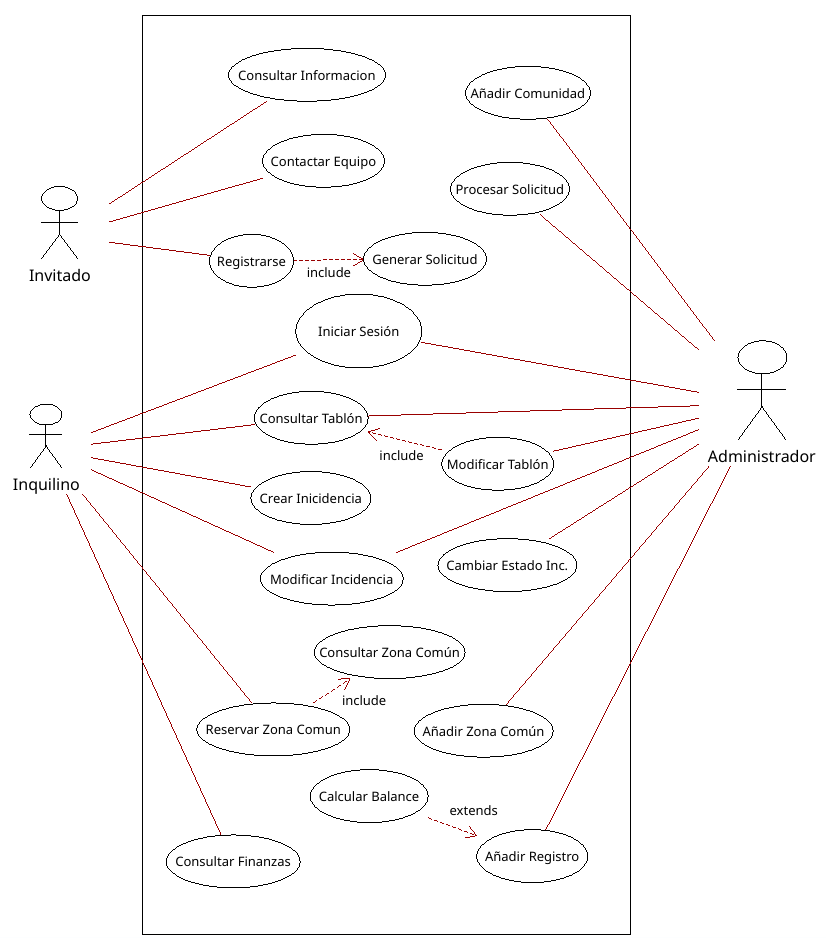
\includegraphics[scale=0.66]{diagrama-CU.png}
	\caption{Diagrama de Casos de Uso General}
\end{figure}

Aunque se han intentado incluir todos los casos de uso, hay alguno se ha quedado fuera, por el bien de la legibilidad del diagrama, aunque han sido casos genéricos. 

En concreto, el \textbf{CU: Consultar Incidencias}, se ha dejado fuera del diagrama, ya que si inclusión disminuía considerablemente la legibilidad de la parte inferior del diagrama, y si rol, dentro de este, es el mismo que el de otros casos de uso similares como \textbf{Consultar Tablón} ó \textbf{Consultar Zona Común}.

\subsection{Descripción Casos de Uso Principales}
En esta sección se van a \textbf{describir}, mediante tablas, los \textbf{casos de uso principales} de nuestro software. 

Hay que tener en cuenta que la \textbf{numeración de los casos de uso} que vemos en las tablas puede no empezar desde 0 o tener números faltantes entre una tabla y otra. Esto se debe a que no todos los casos de uso se van a describir en las tablas y la numeración de estos va acorde a su aparición en el diagrama. Por ejemplo, el primer caso de uso va a ser el \textbf{CU03 - Registrarse}, ya que los primeros 2 casos de uso, \textbf{CU01 - Consultar Información} y \textbf{CU02 - Contactar Equipo} no se van a incluir en esta sección.

\begin{figure}[ht]
	\centering
	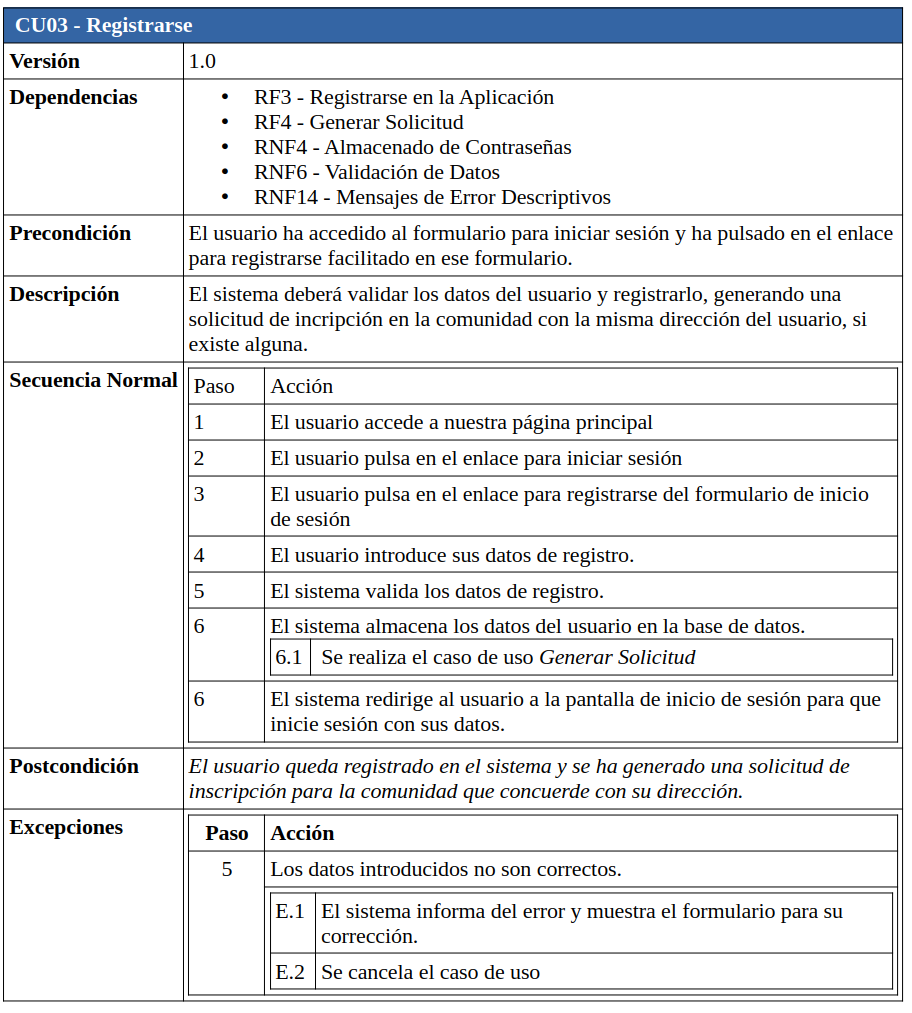
\includegraphics[scale=0.56]{CU03.png}
	\caption{Caso de Uso - Registrarse}
\end{figure}

\begin{figure}[H]
	\centering
	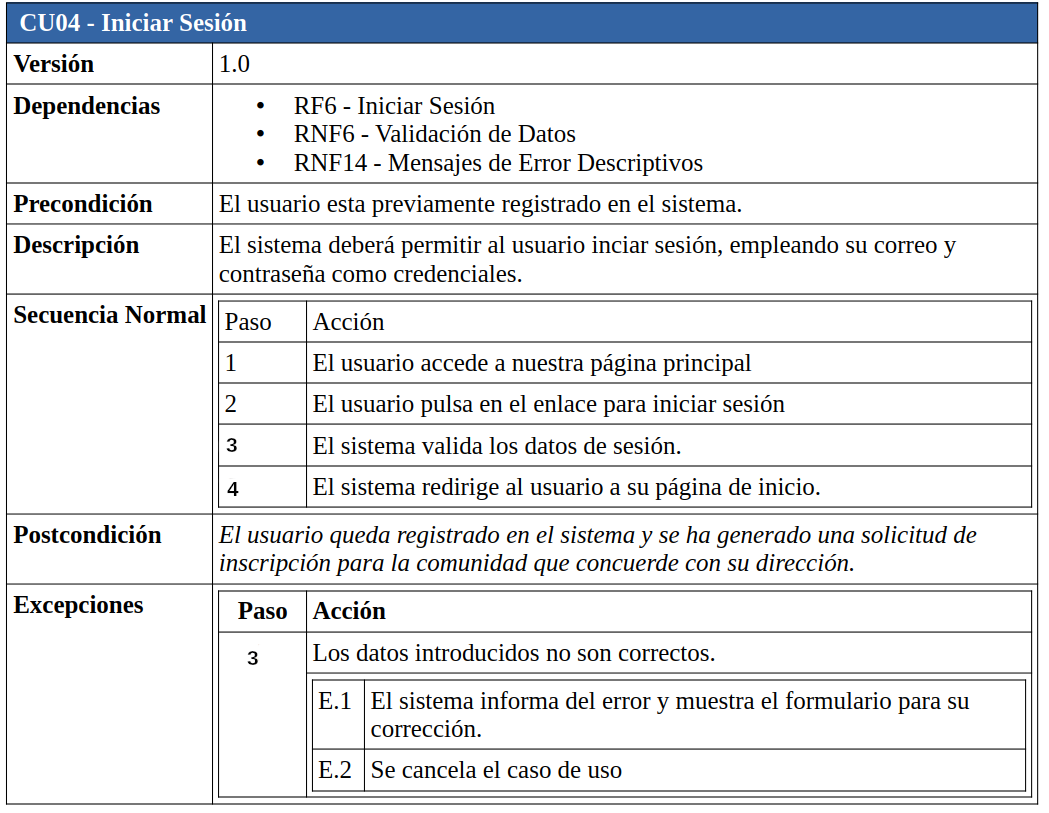
\includegraphics[scale=0.47]{CU04.png}
	\caption{Caso de Uso - Inicio de Sesión}
\end{figure}

\begin{figure}[H]
	\centering
	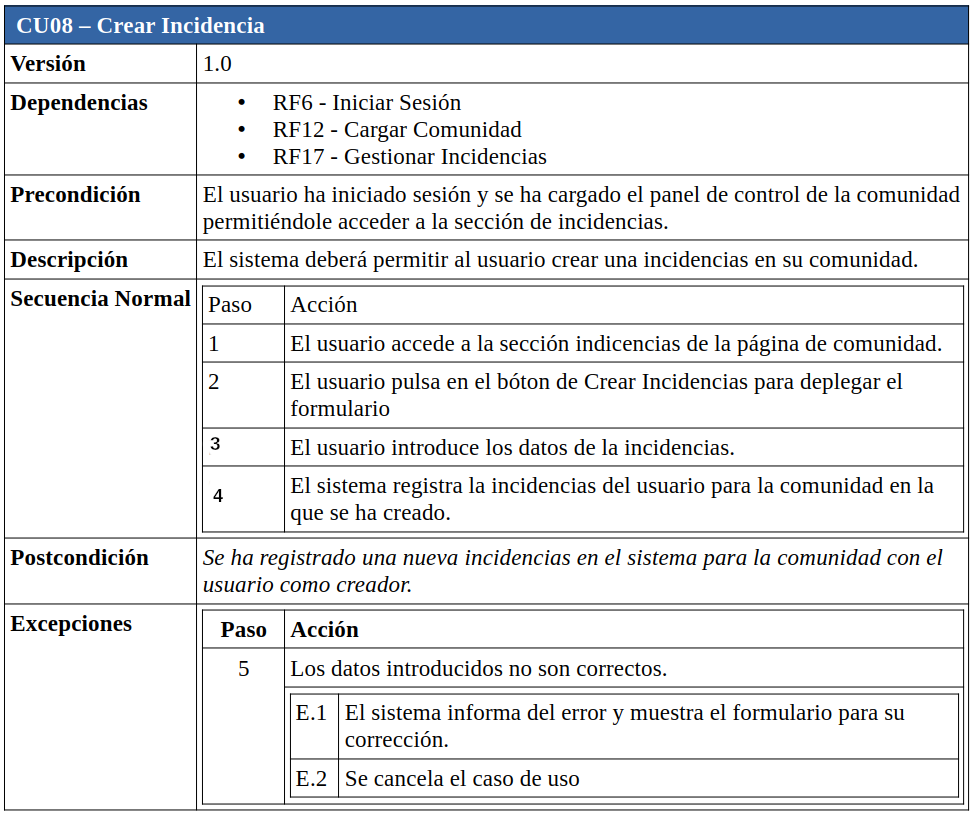
\includegraphics[scale=0.49]{CU08.png}
	\caption{Caso de Uso - Crear Incidencia}
\end{figure}

\begin{figure}[H]
	\centering
	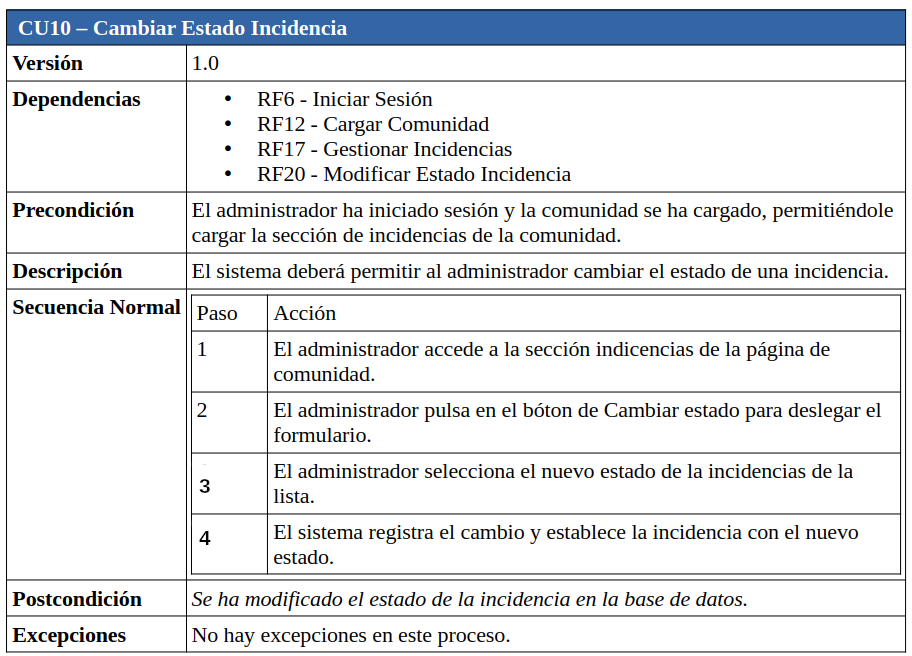
\includegraphics[scale=0.52]{CU10.png}
	\caption{Caso de Uso - Cambiar Estado Incidencia}
\end{figure}

\begin{figure}[H]
	\centering
	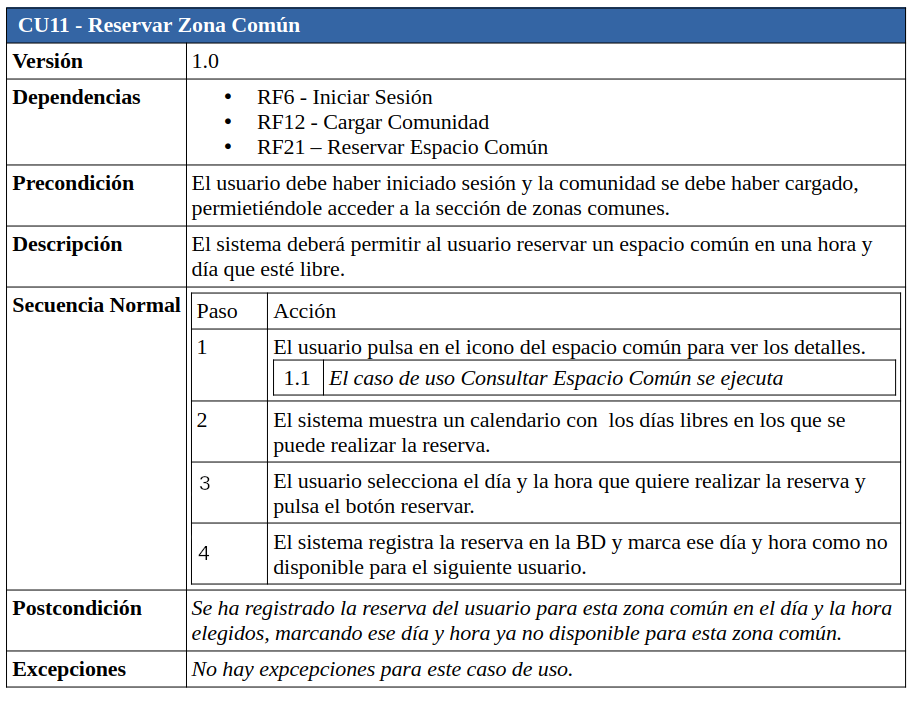
\includegraphics[scale=0.52]{CU11.png}
	\caption{Caso de Uso - Reservar Espacio Común}
\end{figure}

\begin{figure}[H]
	\centering
	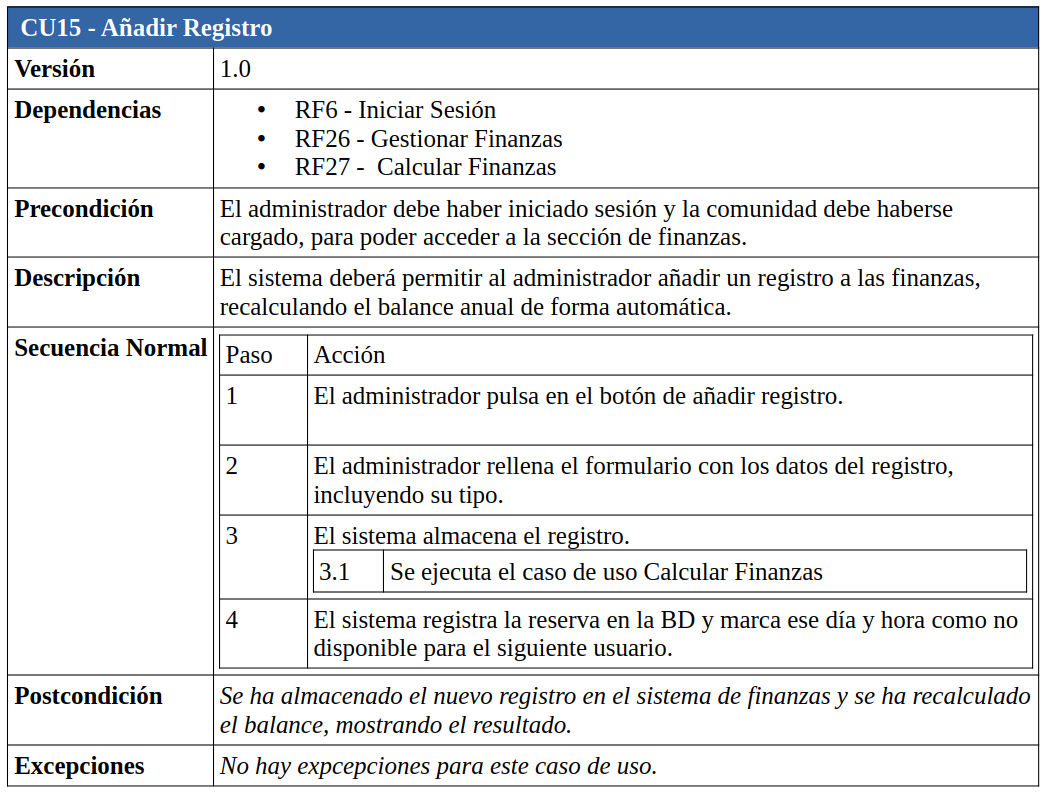
\includegraphics[scale=0.48]{CU15.png}
	\caption{Caso de Uso - Añadir Registro}
\end{figure}


\section{Base de Datos}
En este apartado vamos a describir el \textbf{diseño de la base de datos} que vamos a emplear en nuestra aplicación, mostrando el \textbf{diagrama E/R}, así como su \textbf{paso a tablas}, explicado los puntos que sean necesarios. Además se creará un script para la creación de la base de datos y otro para poblarla con información.

La base de datos de nuestra aplicación es una \textbf{base de datos relacional} que emplea \textbf{SQL} para la realización de las consulta y la creación de la base de datos. La sistema de base de datos elegidos ha sido \textbf{PostgreSQL}, un sistema de gestión de bases de datos objeto-relacional y que pone especial énfasis en la extensibilidad y compatibilidad con SQL. \cite{wiki02}

PostgreSLQ, además, ofrece atomicidad, consistencia, aislamiento, propiedades \gls{ACID}, entre otras cosas. Además es soportada por la mayoría de sistemas operativos y se \textbf{integra perfectamente} con Apache, soportando las versiones de PosgreSQL 7.2.8 o superior. \cite{apache01}

\subsection{Diagrama Entidad/Relación}
En esta sección se muestra el \textbf{diagrama entidad relación} de nuestra base de datos. Como podemos ver en el diagrama, inicialmente hay un total de \textbf{5 tablas}, pero como veremos en la siguiente sección, las relaciones entre estas tablas dan lugar a \textbf{3 tablas más}, que sumarán un total de \textbf{8 tablas}, pero esto ya lo veremos con más detalle en la siguiente sección con el paso a tablas.

Se ha intentado crear la base de datos de la forma más simple posible, \textbf{sin que haya sido necesario normalizarla}.

\begin{figure}[H]
	\centering
	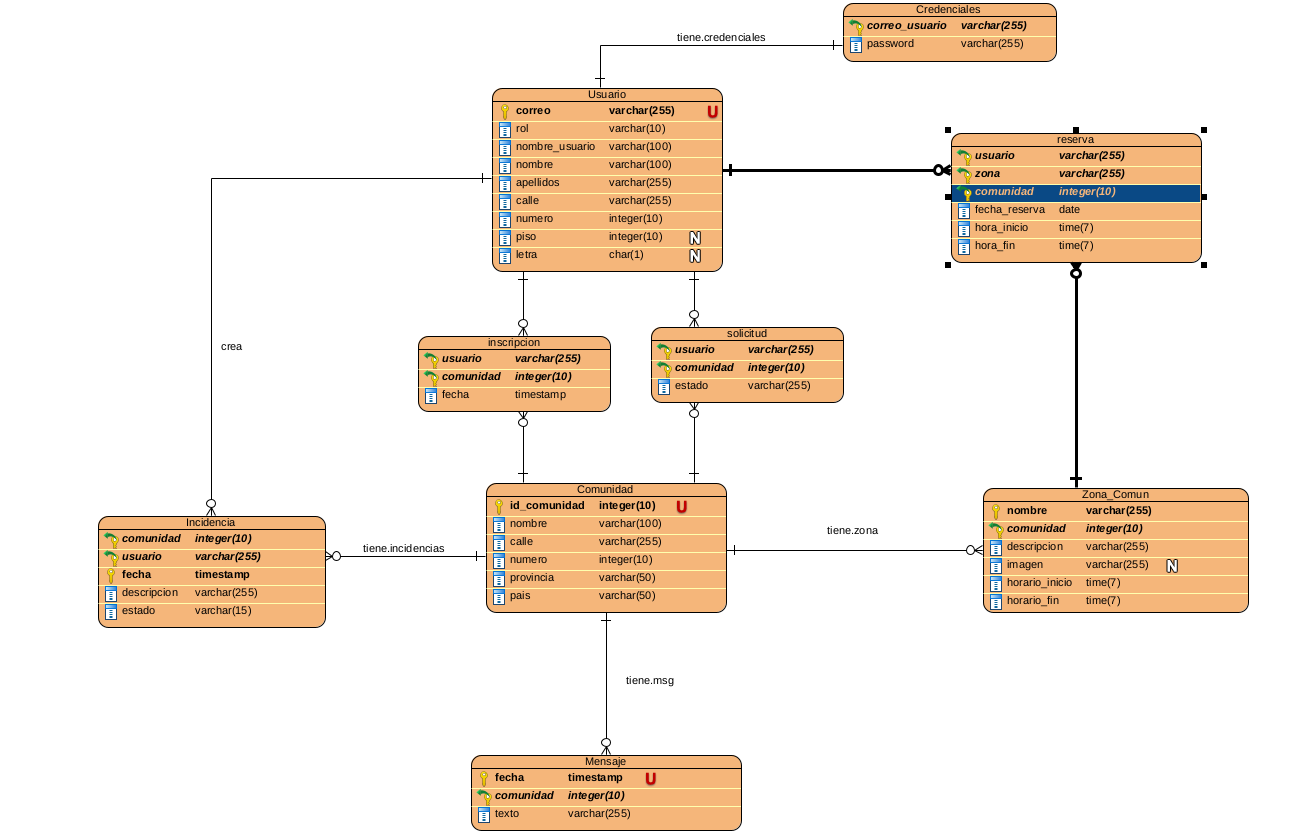
\includegraphics[scale=0.50]{diagramaER.png}
	\caption{Diagrama Entidad/Relación}
\end{figure}

Como vemos, es un diagrama sencillo, donde se ha intentado \textbf{atomizar cada atributo}, además de evitar las referencias circulares. En la siguiente sección veremos el paso a tablas, aunque con este diagrama, donde ya se incluyen como tablas las relaciones, el paso va a ser más directo aún.

\subsection{Paso a Tablas}





\newpage

\appendix

\begin{appendices}
	
\section{Descripción de la Interfaz de Usuario}
\label{sec:apenA}
\textbf{SolucionesVecinales} es una aplicación web, por lo que tendrá una \textbf{interfaz web} que podrá ser accedida desde cualquier navegador y prácticamente desde cualquier dispositivo. La interfaz estará compuesta por un conjunto de páginas web que ayudarán a los usuarios a utilizar los diferentes servicios que ofrece la aplicación para gestionar la comunidad de vecinos. 

Las \textbf{páginas} de las que estará compuesta nuestra interfaz son las siguientes:

\begin{itemize}
	\item \textbf{Página Principal}: está es la página que se carga cuando cualquier usuario entra a nuestra aplicación. La función principal de esta pantalla es la de \textbf{ofrecer información sobre la aplicación}, así como proporcionar un\textbf{ menú con diferentes opciones} que, además de permitir la navegación por las diferentes secciones permita a un invitado \textbf{registrarse} o \textbf{realizar \gls{login}}.
	
	Las secciones de las que estará compuesta esta interfaz serán las siguientes:
	
	\begin{itemize}
		\item \textbf{Cabecera}: aquí se mostrará una imagen con un eslogan, el nombre de la aplicación y un elemento \gls{CTA} para que los usuarios se registren o realicen login.
		
		\item \textbf{Barra de Menú}: esta barra, que se sitúa inicialmente encima de la cabecera y que debe permanecer en todo momento en la parte superior de la pantalla, esta compuesta del \textbf{logo de la aplicación} en el lado izquierdo y de un \textbf{menú} en el lado derecho. El menú estará siempre presente en todas las páginas de la web, aunque dependiendo del contexto, la opción del menú pueden cambiar.
		
		\item \textbf{Secciones}: esta página contendrá, como mínimo, \textbf{3 secciones}, donde se explicará un poco el \textbf{propósito} del software, sus principales \textbf{características}, lo que nos diferencia de la competencia, etc. Las secciones deben ser \textbf{visualmente atractivas}, incluyendo imágenes e iconos y con una disposición adecuada. 
		
		Una sección que deberá ser \textbf{obligatoria}, es la sección ``\textbf{Contacta con nosotros}'', compuesta por un formulario y que permitirá a cualquier usuario, registrado o no, contactar con el equipo de desarrollo.
		
		\item \textbf{Pie de Página}: en el pie de página se añadirá una lista de enlaces con las diferentes secciones de la página, un mapa del sitio web y un conjunto de enlaces de redes sociales de la aplicación o en su defecto del equipo de desarrollo.
	\end{itemize}
	
	Tanto la \textbf{barra de menú} superior como el \textbf{pié de página} se mantendrán \textbf{visibles en todas las páginas} de la aplicación, cambiando en ciertos aspectos u ofreciendo diferentes opciones.
	
	\item \textbf{Página de Login}: el propósito de esta página es permitir que los usuarios ingresen al sistema. La pantalla inicial esta compuesta por un \textbf{formulario}, que debe aceptar un \textbf{email} y una \textbf{contraseña} como entrada, con el botón enviar en la parte inferior. Además, incluirá un \textbf{enlace} debajo del botón, centrado, que permitirá al invitado \textbf{registrarse}, en caso de que no este registrado, desplegando un nuevo formulario que veremos en detalle a continuación. Solo el \textbf{administrador de la web} podrá realizar el ingreso al sistema empleando el \textbf{usuario WebAdmin}, el resto de usuarios deberán usar su correo.
	
	\item \textbf{Página de Registro}: en esta pantalla, que se accede desde la pantalla de login, se muestra un formulario que \textbf{permitirá a un invitado registrarse} en el sistema. Este formulario estará compuesto por diferentes campos que permitirán al invitado introducir la información necesaria pare registrarse, como puede ser Nombre, Correo, Dirección, rol, etc. Debajo, aparecerá el \textbf{botón registrarse} que permitirá al invitado registrar todos sus datos.  

	
	\item \textbf{Página Principal de Comunidad}: una vez que el usuario haya ingresado al sistema, se mostrará la pantalla de comunidad. El propósito de esta pantalla es servir como \textbf{puerta de entrada a la gestión de al comunidad} y como \textbf{punto de información} para el usuario. Esta interfaz estará compuesta por los siguientes elementos:
	
	\begin{itemize}
		\item \textbf{Barra de Menú}: similar a la que vemos en la página principal, pero las opciones de menú ``Login/Registrarse''  habrá cambiado por el \textbf{icono de un usuario}. Este icono mostrará un \textbf{menú vertical} con las opciones ``\textbf{Perfil}'' y ``\textbf{Logout}'', que permitirán acceder a la información de perfil y hacer \gls{logout} respectivamente.
		
		\item \textbf{Menú Lateral}: un menú lateral, situado a la izquierda, que mostrará los diferentes servicios que ofrece al aplicación para gestionar la comunidad. Las opciones variarán según si el usuario tiene el rol de administrador o de inquilino, pero la opciones comunes a ambos son las siguientes: 
		
		\begin{itemize}
			\item \textbf{Inicio}
			\item \textbf{Tablón de Anuncios}
			\item \textbf{Documentos}
			\item \textbf{Incidencias}
			\item \textbf{Espacios Comunes}
			\item \textbf{Finanzas}
		\end{itemize}
	
		 
		 Adicionalmente, si el usuario tiene el \textbf{rol administrador}, se mostrará la opción ``\textbf{Administrar}''	, que permitirá al administrador gestionar los aspectos principales de la comunidad desde una misma pantalla. La cual se describirá más adelante.
		 
		El menú lateral se mostrará solo en caso de que el usuario, independientemente de su rol, este inscrito en una comunidad. En caso contrario no se mostrará. Si es un \textbf{administrador}, se mostrará en su lugar un \textbf{formulario para añadir una comunidad}. Si es un \textbf{inquilino}, se mostrará un \textbf{mensaje con el estado} de su solicitud de suscripción.
		
		\item \textbf{Zona de Contenido}: en esta zona, que estará ubicada en el centro y es el elemento principal de ésta página. Cuando un \textbf{inquilino inscrito en una comunidad} acceda a la página principal de comunidad, aquí se mostrar la \textbf{información} de ésta, como nombre, dirección y una imagen. Además, se mostraran la actividad reciente del usuario, así como otros notificaciones, como las reservas realizadas o el estado de las incidencias creadas.
		
		En esta zona de la interfaz se mostrará todas la información de los diferentes servicios y es donde se permitirá interactuar con la comunidad. Seleccionando alguna de las opciones del menú, los \textbf{principales elementos} que se mostrarán en esta zona y que permiten \textbf{realizar las acciones sobre la comunidad} son las siguientes: 
		
		\begin{itemize}
			\item \textbf{Inicio}: cuando un usuario pinche en esta opción cargara la información por defecto de la página principal de comunidad, que se ha descrito en el párrafo anterior.
			
			\item \textbf{Tablón de Anuncios}: este servicio nos permite acceder a los mensajes que se han publicado en la comunidad y mostrará una lista con todos los mensajes, junto con su fecha. Si \textbf{es un administrador}, aparecerá un botón en la parte inferior izquierda, debajo del tablón, con el texto "\textbf{Añadir mensaje}", que desplegará un formulario que permitirá añadir un nuevo mensaje al tablón de anuncios.	
			
			\item \textbf{Documentos}: pulsando en esta opción se mostrarán los \textbf{documentos relativos a la comunidad}, como pueden ser actas de reuniones, facturas, etc. Los documentos se mostrarán como un conjunto de iconos con un nombre debajo. Tanto el icono como el nombre deberán ser un enlace que al pulsarlo permita a los inquilinos descargar el documento en cuestión. 
			
			En el caso de que el \textbf{usuario sea un administrador}, debe aparecer un botón con el texto "\textbf{Añadir Documento}" que desplegará una formulario y le permitirá añadir nuevos documentos al directorio. 
			
			\item \textbf{Incidencias}: este servicio permitirá a los inquilinos gestionar las incidencias, mostrando una \textbf{lista con todas las incidencias} de la comunidad, junto con su fecha de creación y su estado. Para un \textbf{inquilino}, solo se mostrarán \textbf{sus incidencias} y todos aquellas que hayan sido \textbf{marcadas como públicas} por los inquilinos que las hayan creado. Para el administrador, serán visibles todas las incidencias.
			
			Debajo de la lista de incidencias, debe haber un \textbf{botón} con el texto "\textbf{Crear incidencia}", que desplegará un formulario y permitirá a cualquier usuario crear una nueva incidencia. Además, si el \textbf{usuario conectado es el administrador}, aparecerán 2 botones a la derecha de cada incidencia, que permitirán tanto \textbf{borrar las incidencias} como \textbf{cambiar su estado}. En caso de que el usuario no sea administrador, solo aparecerá el botón ``Borrar'' en las incidencias que hayan sido creadas por él mismo.
			
			\item \textbf{Zonas Comunes}: se mostrarán las diferentes zonas comunes de la comunidad y se permitirá su reserva. Se mostrará un icono por cada zona, con todos los espacios comunes que hay en al comunidad, que permitirá clickar en ellos y acceder a la página de cada espacio común. Además, para los administradores, se mostrará un botón con el texto ``Añadir Espacio'' que mostrará un formulario que permitirá añadir un nuevo espacio común, con información como el nombre del espacio común, sus características y el horario de uso, además de la posibilidad de incluir una foto de dicho espacio.
			
			\begin{itemize}
				\item \textbf{Detalle de Zona Común}: se muestran los \textbf{detalles de una zona común}. Aparecerá \textbf{una imagen}, si se hubiera incluido. Sino se cargara una imagen por defecto. Encima aparecerá el \textbf{nombre} del espacio común y al lado derecho de la imagen, una \textbf{descripción} de dicho espacio. Debajo de la descripción aparecerá el horario de uso de dicho espacio.
				
				Debajo de este bloque, se mostrará un \textbf{calendario}. Los \textbf{días en los que no se pueda reservar} tendrán un fondo \textbf{rojo} y en los que aún \textbf{si se pueda} tendrán un \textbf{fondo verde}. Al \textbf{pinchar} sobre uno de estos días se desplegará una \textbf{lista con los posibles horarios} en los que se puede reservar, permitiendo pinchar en uno y pulsar el \textbf{botón "Reservar"} que habrá también aparecido junto con los horarios.
			\end{itemize}
			
			\item \textbf{Finanzas}: se mostrará una \textbf{tabla con las finanzas} de la comunidad, indicando los ingresos y el tipo de estos, como cuotas, seguros, etc., así como los gastos y su tipo, limpieza del edificio, arreglos, seguros, etc. La información de mostrará para este ejercicio, realizando una estimación, y se irá modificando de forma automática cuando se añadan gastos o ingresos, aunque también se podrá consultar para ejercicios anteriores. 
			
			Solo los \textbf{administradores} puede modificar esta tabla, mediante un formulario para añadir un registros en el que se podrá seleccionar el tipo de registro, si es un ingreso o gasto, y el tipo de cada uno, así como la cantidad. Cuando se agregue un nuevo registro, el sistema calculará el balance con los nuevos datos y los mostrará. Este formulario se mostrará después de pulsar el botón ``Añadir'' debajo de la tabla de finanzas. Solo se pueden añadir o borrar registros en el ejercicio actual.
			
			\item \textbf{Administrar}: esta opción solo es elegible por los \textbf{administradores} y permite al administrador \textbf{gestionar} todos los aspectos de una \textbf{comunidad} mediante un panel de control.
			
			En la zona de contenido se mostrará \textbf{información de al comunidad}, que será editable, así como los servicios mencionados en este punto: Incidencias, Documentos, Finanzas, etc., con opciones para editar, consultar añadir o eliminar elementos a cada apartado. Los apartados se mostrarán uno al lado de otro con iconos y al pulsar en ellos se desplegará una lista con todos los elementos que estos contienen, ocultando el resto secciones. Además aparecerá un botón para poder volver hacia atrás a la lista de servicios.
						
			\item \textbf{Barra de Búsqueda}: cabe destacar que \textbf{todas las secciones} incluirán, encima de la tabla o lista donde se muestra la información, una \textbf{barra de búsqueda} que permitirá seleccionar solo las entradas coincidentes con los términos que queramos.
		\end{itemize}
	\end{itemize}
		
	
	\item \textbf{Página de Añadir Comunidad}: esta pantalla, a la que solo tienen acceso los administradores, permite \textbf{añadir una nueva comunidad} de vecinos. La interfaz mostrará un \textbf{formulario web} con diferentes datos que deberán rellenarse para dar de alta la comunidad, principalmente la \textbf{dirección}, que será única para cada comunidad. En el caso de que se pueda dar de alta la comunidad se mostrará una mensaje de éxito y se redireccionará a la página principal de comunidad. En caso contrario, se mostrará los mensajes de error adecuados.
	
	\item \textbf{Página de Perfil}: en esta pantalla, que se accede desde el menú vertical del icono de perfil, se mostrará un \textbf{formulario con toda la información del usuario} en la zona de contenido. Este formulario se podrá \textbf{editar} y actualizar mediante un botón que habrá debajo de él con el texto "Guardar". 
	
	Además, debajo de este aparecerá un \textbf{botón} con la opción ``\textbf{Eliminar usuario}'' que permitirá a un usuario eliminar su información, y que al ser pulsado ocultará el formulario con al información y mostrará una ventana de confirmación. Si la confirmación es positiva, se eliminará al usuario, y se redireccionará la pantalla principal.
	
	\item \textbf{Backoffice}: esta es una interfaz especial, ya que solo es accesible por el \textbf{administrador web} o \textbf{WebAdmin} y sirve como un punto centralizado para gestionar todos los servicios y consultar datos sobre la aplicación.
	En la parte superior aparecerá un tabla con \textbf{estadísticas} de uso generales de la aplicación. Debajo de esta tendremos un formulario con diferentes opciones para generar informes más específicos que se mostrarán en la tabla de superior.
	
	Debajo de este apartado, aparecerán \textbf{dos iconos}, uno para \textbf{las comunidades} y otro para \textbf{los usuarios}. Al pulsarlo, aparecerá una pantalla con una lista desplegable, con todas las comunidades registradas en al aplicación. Al pulsar en una comunidad, se desplegará una lista mostrando los usuarios registrados en al comunidad, el administrador y los espacios comunes registrados, el número de documentos, etc. En el caso de los usuarios se mostrará una tabla con todos los usuarios registrados en al aplicación.
	
	Dentro de las pantallas de comunidad y usuarios, el \textbf{WebAdmin} podrá \textbf{añadir} o \textbf{eliminar} cualquier comunidad o usuario. También se podrán eliminar servicios dentro de una comunidad.
\end{itemize}

Además de estas páginas, hay que tener en cuenta que la aplicación debe \textbf{visualizarse correctamente en cualquier dispositivo}. Aunque se añadirán restricciones más adelante en este aspecto, hay que tener en cuenta que algunos \textbf{elementos cambiarán} cuando la aplicación se visualice en \textbf{dispositivos pequeños}, como móviles o tablets. Estos elementos son:

\begin{itemize}
	\item \textbf{Barra Superior}: en la barra superior todas las opciones del menú se agruparán en un \gls{menú hamburguesa}, el cual se situará en la parte derecha de la barra.
	
	\item \textbf{Menú Lateral}: el menú lateral se ocultará, mostrando la interfaz una flecha en la parte superior izquierda, donde debería estar el menú. Al pulsar esta flecha 
\end{itemize}

Más adelante, en la sección de adecuación al entorno y restricciones de diseño se proporcionará más información sobre el desempeño de la aplicación en dispositivos móviles y tablets.

\newpage

\section{Tablas de Requisitos}
\label{sec:apenB}
En este anexo se incluyen varias tablas con los requisitos funcionales y no funcionales, ya que son muy extensas se ha preferido dividir éstas para no hacer tablas que ocupen varias páginas.

\begin{table}[H]
	\begin{center}
		\bgroup
		\def\arraystretch{1.5}
		\begin{tabular}{| p{5cm} | p{10cm} |}
			\hline
			\textbf{Número y Tipo} & \textbf{Descripción}  \\ \hline
			RF1.- Consultar Web Principal &  Cualquier usuario podrá acceder a la página web principal para consultar la información sobre nuestra aplicación \\ \hline
			RF2.- Contactar Equipo & Cualquier usuario podrá contactar con el equipo de desarrollo usando
			el formulario de la página principal, dejando un mensaje y su correo \\ \hline
			RF3.- Registrarse en la Aplicación & Los invitados podrán registrarse en nuestra aplicación empleando el formulario de la página de registro e introduciendo su correo, nombre, apellidos, nombre
			de usuario y dirección  \\ \hline
			RF4.- Generar Solicitud & El sistema deberá generar una solicitud de inscripción en la comunidad que coincida con la dirección que ha especificado el invitado que se ha registrado  \\ \hline
			RF5.- Aprobar Solicitud: & El administrador de la comunidad deberá poder aceptar o denegar la
			solicitud de inscripción en la comunidad de un invitado  \\ \hline
			RF6.- Iniciar Sesión & Un inquilino o administrador podrá ingresar al sistema empleando su correo
			y contraseña como credenciales  \\ \hline
			RF7.- Añadir Comunidad & El administrador podrá añadir una nueva comunidad de vecinos, independientemente de que 
			este inscrito ya en alguna otra, especificando un nombre, descripción, imagen y dirección de la comunidad  \\ \hline
			RF8.- Modificar Perfil &  Un inquilino o administrador podrá acceder a su perfil y modificar sus datos
			en el sistema \\ \hline
			RF9.- Eliminar Usuario & Un inquilino podrá eliminar su usuario desde su página de perfil, pudiendo
			ser también eliminado por el administrador  \\ \hline
			RF10.- Eliminar Administrador & El administrador podrá eliminar su información desde su página de perfil, siempre y cuando no este adscrito a ninguna comunidad  \\ \hline
			RF11.- Eliminar Comunidad &  El administrador podrá eliminar una comunidad de vecinos, que
			haya creado, desde la sección para administrar la comunidad  \\ \hline
			RF12.- Cargar Comunidad & Cuando un inquilino o administrador inicie sesión, se cargará la página
			principal de la comunidad mostrando los datos de ésta, así como las notificaciones del usuario  \\ \hline
			RF13.- Notificar Usuario &  El sistema creará notificaciones con los documentos descargados en
			los últimos 10 días, las reservas de espacios comunes y las incidencias de un usuario, mostrándolos
			en la página principal de la comunidad  \\ \hline
		\end{tabular}	
		\egroup
		\caption{Requisitos Funcionales (Parte I)}	
	\end{center}
\end{table}  

\begin{table}[H]
	\begin{center}
		\bgroup
		\def\arraystretch{1.5}
		\begin{tabular}{| p{5cm} | p{10cm} |}
			\hline
			\textbf{Número y Tipo} & \textbf{Descripción}  \\ \hline
			RF14.- Consultar Tablón & Un inquilino o administrador podrá consultar los mensajes creados en
			el tablón de anuncios \\ \hline
			RF15.- Gestionar Tablón & El administrador podrá crear o eliminar mensajes del tablón de anuncios de la comunidad \\ \hline
			RF16.- Consultar Documentos &  Un inquilino podrá consular los documentos relativos a la comunidad y descargarlos a su dispositivo\\ \hline
			RF17.- Gestionar Documentos & El administrador podrá añadir o eliminar documentos de una comunidad \\ \hline
			RF18.- Consultar Incidencias &  Un inquilino podrá consultar las incidencias publicas o creadas por
			el mismo, mientras que una administrador podrá consultar todas las incidencias relativas a una
			comunidad \\ \hline
			RF19.- Gestionar Incidencias & Un inquilino podrá crear incidencias, así borrar o modificar las incidencias creadas por
			el mismo, mientras que el administrador podrá eliminar las incidencias de cualquier usuario \\ \hline
			RF20.- Modificar Estado de Incidencia &  El administrador podrá cambiar el estado de las incidencias entre: “Creada”, “En Proceso” y “Resuelta”\\ \hline
			RF21.- Añadir Espacio Común & El administrador podrá añadir espacios comunes especificando
			su nombre, descripción y horario de reserva \\ \hline
			RF22.- Reservar Espacio Común & Un inquilino podrá reservar un espacio común seleccionando
			en un calendario el día y hora que quiere realizar la reserva, siempre y cuando este libre \\ \hline
			RF23.- Cancelar Reserva & Un inquilino podrá cancelar una reserva de un espacio común desde la
			sección de espacios comunes o desde la página principal de la comunidad  \\ \hline
			RF24.- Gestionar Espacios Comunes &  El administrador podrá eliminar o modificar la información relativa a un espacio común \\ \hline
			RF25.- Consultar Finanzas & Un inquilino podrá consultar las finanzas de la comunidad en la sección finanzas que se mostrarán en una tabla con los datos estimados para el curso actual, pudiendo
			 también consultar los datos del curso anterior \\ \hline
			RF26.- Gestionar Finanzas &  El administrador podrá añadir, eliminar o modificar los registros de
			la tabla de finanzas\\ \hline
			RF27.- Calcular Finanzas & El sistema realiza el calculo de las finanzas cada vez que se añada o
			elimine un pago o un ingreso \\ \hline
			RF28.- Cerrar Sesión &  Un inquilino o administrador podrán cerrar la sesión en el sistema desde el
			icono de usuario \\ \hline
			RF29.- Administrar Servicios & el administrador web podrá iniciar sesión empleando el usuario
			WebAdmin y acceder al panel de control para administrar los diferentes servicios web así como
			para obtener datos de uso de la aplicación \\ \hline
		\end{tabular}	
		\egroup
		\caption{Requisitos Funcionales (Parte II)}
	\end{center}
\end{table}  

\begin{table}[H]
	\begin{center}
		\bgroup
		\def\arraystretch{1.5}
		\begin{tabular}{| p{5cm} | p{10cm} |}
			\hline
			\textbf{Número y Tipo} & \textbf{Descripción}  \\ \hline
			RNF1.- Arquitectura & La aplicación se implementará empleando una arquitectura cliente-servidor \\ \hline
			RNF2.- Protocolo Comunicación &  La aplicación empleará el protocolo HTTPS entre el cliente y
			el servidor, no permitiendo conexión con otro protocolo que no sea este\\ \hline
			RNF3.- Peticiones Limitadas & Las peticiones por segundo al servidor estarán limitadas a 10, para
			evitar ataques de tipo DOS \\ \hline
			RNF4.- Almacenado de Contraseñas &  El sistema se encargará de almacenar las contraseñas en la
			base de datos de forma segura, nunca en texto plano, empleando un algoritmo hash y almacenando
			el resultado encriptado en la base de datos\\ \hline
			RNF5.- Robustez Contraseñas &  El sistema solo aceptará contraseña con un mínimo de 12 caracteres y con al menos un número y un signo de puntuación\\ \hline
			RNF6.- Validación de Datos &  Los datos introducidos por los usuarios serán validados tanto en el
			cliente como en el servidor\\ \hline
			RNF7.- Tiempo de Carga &  La aplicación deberá tener un tiempo de carga en el navegador del
			usuario inferior a 3 segundos\\ \hline
			RNF8.- Compresión Archivo Multimedia & Los archivos multimedia empleados en la web deberán estar comprimidos lo máximo posible sin que estos pierdan calidad significativamente\\ \hline
			RNF9.- Uso de Memoria &  El cliente de nuestra aplicación deberá usar el mínimo de memoria
			posible para cumplir su función de forma eficiente\\ \hline
			RNF10.- Interfaz Adaptable &  El cliente de nuestra aplicación deberá tener una interfaz que se
			adapte a diferentes dispositivos, incluyendo dispositivos móviles y tablets\\ \hline
			RNF11.- Alternativa Textual &  Cualquier elemento de la interfaz que no sea texto deberá tener
			una alternativa textual\\ \hline
			RNF12.- Contraste &  La interfaz tiene que tener un contraste mínimo entre el texto y el fondo de
			4.5:1 para textos pequeños y 3:1 para textos grandes\\ \hline
			RNF13.- Navegabilidad &  La interfaz deberá ser totalmente navegable con el teclado\\ \hline
			RNF14.- Mensajes de Error Descriptivos &  Cualquier mensaje de error que produzca la aplicación, ya sea para los usuarios o desarrolladores, debe explicar correctamente por qué se ha producido el error\\ \hline
			RNF15.- Test Unitarios & Todo componente, función o clase deberá tener implementando su correspondiente test unitario \\ \hline
			RNF16.- Cobertura de Tests &  Los test deberán cubrir el 100\% del código desarrollado\\ \hline
		\end{tabular}	
		\egroup
		\caption{Requisitos No Funcionales (Parte I)}
		\end{center}
\end{table}

\begin{table}[H]
	\begin{center}
		\bgroup
		\def\arraystretch{1.5}
		\begin{tabular}{| p{5cm} | p{10cm} |}
			\hline
			\textbf{Número y Tipo} & \textbf{Descripción}  \\ \hline
			RNF17.- CD/CI &  Los test unitarios, así como los e2e y los de integración deberán ejecutarse con
			un sistema de integración/despliegue continuo\\ \hline
			RNF18.- Calidad Global del Código &  La calidad global del código debe garantizarse, empleando
			para ellos herramientas como Code Climate, eslint y todas aquellas que sean necesarias para que
			el código se adapte a las buenas prácticas y estándares\\ \hline
			RNF19 - Formato del Código & El código se formateará empleando prettier, con una configuración
			predefinida para que todo el código, de cualquier desarrollador, tenga el mismo formato \\ \hline
			RNF20 - LOPD y RGPD & En cumplimiento de las leyes LODP y RGPD, deberán mostrarse a los
			usuarios los documentos legales siguientes: Política de Privacidad y Política de Cookies \\ \hline
		\end{tabular}	
		\egroup
		\caption{Requisitos No Funcionales (Parte I)}
	\end{center}
\end{table}

\end{appendices}

\newpage

\printglossary	

\newpage

\bibliography{citas}
\bibliographystyle{unsrt}

\end{document}